\documentclass[twoside]{article}
\usepackage{ecj,palatino,epsfig,latexsym,natbib}
%\usepackage[fleqn]{amsmath}
\usepackage[ruled,vlined]{algorithm2e}
\usepackage[noend]{algpseudocode}
\usepackage{amssymb}
\usepackage{amsmath}
\usepackage{subcaption}
\usepackage[super]{nth}
\usepackage{graphicx}
\graphicspath{{./img/}}
\DeclareGraphicsExtensions{.eps,.jpeg,.png}

\newcommand{\argmax}{\operatornamewithlimits{argmax}}
\newcommand{\argmin}{\operatornamewithlimits{argmin}}

%% do not add any other page- or text-size instruction here

\parskip=0.00in

\begin{document}

\ecjHeader{x}{x}{xxx-xxx}{200X}{Multi-armed Bandit Based Evolutionary Model Adaptation}{CY Hsu, TL Yu and JH Wu}
\title{\bf Multi-armed Bandit Based Evolutionary Model Adaptation for Permutation Problems}  


\author{\name{\bf Chu-Yu Hsu} \hfill \addr{r01921096@ntu.edu.tw}\\ 
        \addr{Department of Electrical Engineering, National Taiwan University, 
         Taipei, Taiwan}
\AND
       \name{\bf Tian-Li Yu} \hfill \addr{tianliyu@ntu.edu.tw}\\
        \addr{Department of Electrical Engineering, National Taiwan University, 
         Taipei, Taiwan}
\AND
       \name{\bf Jia-Hui Wu} \hfill \addr{r02921074@ntu.edu.tw}\\
        \addr{Department of Electrical Engineering, National Taiwan University, 
         Taipei, Taiwan}         
}

\maketitle


%\begin{abstract}

This paper has provided a framework of model adaptation for estimation of distribution algorithms (EDA) on permutation problems. Characterized by the use of probabilistic models to represent the solutions and the dependencies between the variables of the problem, EDAs are known as powerful evolutionary algorithms that have been widely used for diverse types of problems. However, since the semantics of permutation problems differs, each model developed for EDAs can only deal with a subset of permutation problems. The performance suffers from inappropriate model choice. Furthermore, permutation problem may go beyond the existing models can handle. Motivated by these difficulties mentioned above, several model adaptation frameworks, which incorporate multiple models and dynamically decide to use which model, are trialled. In the first trial, the enumeration method samples multiple models simultaneously and shows better performance on Linear Ordering Problem. To reduce the waste of sampling unpromising models, the Bayesian method has been proposed characterized by measuring the quality of each model. However, the Bayesian method tends to choose inappropriate model because of the selection and the template mechanism. Considering the similarity between model adaptation and multi-armed bandit problem, a multi-armed bandit based model adaptation framework has been proposed. In order to prove the potential of the proposed framework, different permutation problems have been tested. The result shows that the proposed framework outperforms the other single model EDA on problems that do not have dedicated models like the vehicle routing problem with time window, and is close to the EDAs with dedicated models on the specific problem like the traveling salesman problem. 

\end{abstract}

\begin{keywords}
Estimation of distribution, 
permutation problem, 
model adaptation, 
multi-armed bandit problem.

\end{keywords}

%\section{Introduction}
\label{ch:introduction}

%介紹 - 1. EDA的發展, 2. Permutation Problem的分歧性, 3. EDA for permutaitons
% 4. MAB 5. Road Map 
Estimation of distribution algorithms (EDAs)~\citep{lozano2006towards, larranaga2002estimation, pelikan2002survey, Hauschild2011} constitute a powerful Evolutionary Algorithm (EA) tool for optimization. The main characteristic of EAs is the use of techniques inspired by the natural evolution of the species. In nature, species change across time; individuals evolve, adapting to the characteristics of the environment. This evolution leads individuals with better characteristics. EDAs are stochastic optimization techniques that explore the space of potential solutions by building and sampling explicit probabilistic models of promising candidate solutions. This model-based approach to optimization has allowed EDAs to solve many large and complex problems. The same idea is translated to the realm of computation, where an individual presents a particular solution for the problem to be solved, a population comprises several individuals, and different operators such as crossover, mutation and selection techniques which are used to make the individuals (solutions) evolve. The most popular reference of these types of algorithms are the Genetic Algorithms (GAs)~\citep{Goldberg:1989:GAS:534133}.

Along the development of GAs, EDAs were introduced in the field of EAs in~\citep{muhlenbein1996recombination}. Different from GAs, EDAs learns a joint probability distribution associated with the set of most promising individuals at each generation, trying to explicitly express the interrelations between the different variables of the problem. Sampling the probabilistic model generated in the previous generation, a new population of solutions for the problem is generated. The algorithm stops iterating and returns the best solution found across the generations when a certain stopping criterion is met, such as maximum number of evaluation (NFE), homogeneous population, or lack of improvement in the solutions.

The general EDA framework begins with the initialization stage, which randomly generates a initial population. Next, the evaluation stage calculates the fitness of each individual. The fitness represents the quality of a individual. The selection stage selects a set of individuals outperforming the others. Then, in the model building stage, the probabilistic model is built with the selected individuals. The sampling stage generates the offspring with the model just built. In the replacement stage, the offspring replace the original population. Then, evaluate the individuals again and repeat this flow until meet the terminate criterion. Algorithm \ref{alg:eda} introduces a pseudo-code of EDAs.

\begin{algorithm}[t]
    generate initial population $P$\;
    \While{not meet the terminate criterion}{
        select population of promising solution $S$\;
        build probabilistic model $M$ for $S$\;
        sample $M$ to generate offspring set $O$\;
        incorporate $O$ into $P$\;
    }
    \caption{Estimation of distribution algorithm (EDA)}
    \label{alg:eda}
\end{algorithm}

Based on this general framework, several EDA approaches have been developed in the last years~\citep{Harik1999, pelikan2005hierarchical, Yu2009}, where each approach learns a specific probabilistic model that conditions the behavior of the EDA from the point if view of complexity and performance. Many works in the literature confirm the good performance of EDAs in the solution of problems from diverse fields. Protein Folding~\citep{santana2008protein}, Capacitated Vehicle Routing Problems~\citep{tsutsui2004solving}, Calibration of Chemical Applications~\citep{mendiburu2006parallel}, Treatment Optimization for Cancer~\citep{brownlee2008application} or Nuclear Reactor Fuel Management Parameter Optimization~\citep{jiang2006estimation} are some examples of many real-world problems where EDA-based approaches were applied to find optimal solutions.

In the past decades, the literature have been interested in the solution of a specific subset of NP-hard optimization problems~\citep{ceberio2012review, bosman2001crossing, tsutsui2002probabilistic, tsutsui2006node, ceberio2011introducing, ceberio2013plackett, pelikan2007dependency}. Particularly, those problems whose solutions can be naturally represented as a permutation. In combinatorics, a permutation is understood as a vector $\sigma = (\sigma_1,..., \sigma_n)$ of the indices ${1,...,n}$ such that $\sigma_i \neq \sigma_j$ for all $i \neq j$. Index $j$ is in position $i$ in $\sigma$ when $\sigma_i = j$.

In this paper, this kind of problems are referred as permutation problem. In some problems, solution quality depends mainly on the relative ordering of pairs of permutation elements and the task is to find a permutation to satisfy a set of relative-ordering constraints; an example problem of this type is job-scheduling~\citep{taillard1993benchmarks, johnson1954optimal}. Sometimes solution quality depends mainly on the pairs of elements that are located next to each other (neighbors), which is a typical feature of the traveling salesman problem~\citep{goldberg1985alleles}and similar problems. Since the semantics differs from problem to problem, many models are proposed for different kind of permutation problems~\citep{tsutsui2002probabilistic, tsutsui2006node, ceberio2011introducing, ceberio2013plackett, tsutsui2006edge, tsutsui2006comparative}. 

In~\citep{tsutsui2002probabilistic}, Tsutsui proposed a model named Edge Histogram Matrix which learns the adjacency of the indices. The experiment shows promising results that algorithms with Edge Histogram Matrix outperform on the traveling salesman problem. In~\citep{tsutsui2006node}, Node Histogram Matrix models the absoluter position of indices which performs well on the quadratic assignment problem. Since a model can only deal with a subset of permutation problems, models keeps being proposed and being design. But the semantics of more permutation problems are complicated, like the permutation flow-shop problem and the capacitated vehicle routing problem with constraints.
 
This paper aims to incorporate different permutation models and make them work together. The proposed framework in this paper makes models cooperate with ease. The technique for multi-armed bandit problems is introduced in the proposed framework. Multi-armed bandit problems have been introduced by Robbins~\citep{robbins1985some} and have since been used extensively to model the tradeoffs faced by an automated agent which aims to gain new knowledge by exploring its environment and to exploit its current, reliable knowledge~\citep{robbins1985some, Kuleshov2000, Mohri2005}.

In order to study the efficiency of the multi-armed bandit based model adaptation, we deal with several different problems, the linear ordering problem, the permutation flow-shop scheduling problem, the capacitated vehicle routing problem, the traveling and so on. we compare the results with those obtained by other EDAs for permutation problem.

The remainder of this paper is organized as follows. In the first section, the permutation problems are defined more specifically. Section \ref{ch:related_works} describes several permutation models in detail. Section \ref{ch:essence_of_adaptation} indicates the essence of model adaptation. Next, Section \ref{ch:methodology} discusses several model adaptation approaches, and lists experiment results. the multi-armed bandit based model adaptation is also introduced in this section. Finally, some conclusions and future work ideas are presented in Section \ref{ch:conclusion}.

\begin{abstract}

\end{abstract}
\section{Introdution}
%\section{Permutation Problems}
%\section{Existing Semantic Models For Permutation Problems}
\section{Permutation Problems}
\label{ch:permutation_problems}

Because of different semantics of permutation problems, the understanding of the permutation problem is helpful for designing the model for solving the permutation problem and learning the difficulty that EDAs for the permutation problem encounter. In the following sections, we give an brief introduction to five typical examples of permutation problems, where although the encoding of the solution is given by permutations, the semantics in each case is different.

\subsection{Traveling Salesman Problem}

The traveling salesman problem (TSP)~\citep{goldberg1985alleles} which is a well-known NP-Complete problem. looks for the shortest path, in terms of time, distance, or any similar criterion, to go over $n$ different cities visiting each city only once and returning to the city of departure. A solution is usually given by a sequence of cities represented as a permutation. The search space is denoted as a permutation.
In a TSP instance of 4 cities, $\pi = (3,2,4,1)$ would be a possible solution, indicating that the initial city is 3, then 2, 4, 1, finally coming back to 3. As we assume that the first city of the path is not fixed, TSP is a problem with cyclic solutions, and each solution can be represented by $2n$ different permutations for symmetric instances and $n$ for asymmetric instances. For instance, the solution ${\pi}'=(1,3,2,4)$ represents the same city-tour that $\pi$ does, while the permutations are different.

The objective function $F$, is defined as the sum of the distances of going from city $i-1$ to $i$, denoted as $d_{ij}$, through all cities in the order specified by the permutation:
\begin{equation*}
	F(\pi_1, \pi_2, ... , \pi_n) = \sum_{i=2}^{n}{d_{\pi_{i-1}\pi_i}} + d_{\pi_n\pi_1} \text{.}
\end{equation*}

In TSP we note that the relevant information for the calculation of the fitness function of a solution is given by the relative ordering of the indices in the permutation. The information drawn from the absolute positions of each index is useless, as stated with $\pi$ and ${pi}'$. Furthermore, no matter which position indices $i$ and $j$ are in the permutation, if they are adjacent, the contribution to the objective function is the same.

\subsection{Capacitated Vehicle Routing Problem}
\label{section:cvrp}
The vehicle routing problem (VRP) is an NP-hard combinatorial optimization problem which is introduced in~\cite{dantzig1959}. VRP involves a fleet of vehicles which supply customers with parcels.
Besides, VRP is a most generalized version of TSP. The capacitated vehicle routing problem (CVRP)~\cite{toth2001vehicle} is the most basic variant of the standard VRP. In this variant, the vehicles have a maximum capacity. The vehicles are based at a depot, or hub, from where they must begin and end their route. Customers are located at given points on a map. Each vehicle has a given capacity and each customer has a given demand. The delivery must be accomplished by finding optimal routes which result in a minimal total distance.

Let $C$ be delivery capacity of each vehicle, $L_i$ be the length of the route of vehicle $i$, $W_i$ be the total weight of the parcels assigned to vehicle $i$, and $N_v$ be the number of vehicles. Then the capacitated vehicle routing problem can be formulated as follows:
\begin{eqnarray*}
    \text{Minimize } L=\sum_{i=1}^{N_v}{L_i} \\
    \text{Subject to } W_i \leq C \text{for each} i = 1,2,...,N_v
\end{eqnarray*}

The encoding method for CVRP basically follows the method used in~\citep{tsutsui2004solving}. The vehicles and the customers are encoded into a fixed size permutation. In the permutation, the node numbers $0,1,2...,N_c-1$ are assigned for each customer, and node numbers $N_c, N_c+1, N_c+2,...,N_c+N_v-2$ are assigned for route dividing, where $N_c$ is the number of customers. Hence, $N_v-1$ different node numbers are used as virtual nodes for route dividing.

\begin{figure}[t]
    \centering
    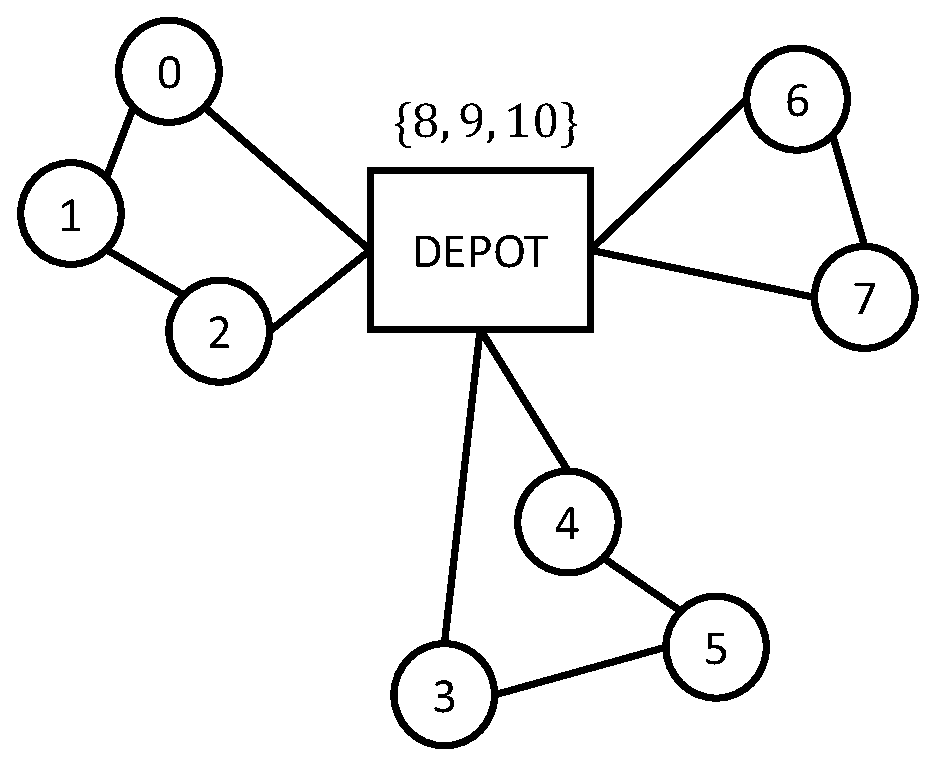
\includegraphics[width=0.5\textwidth]{cvrp_encoding.eps}
    \caption{Permutation Representation of CVRP, $N_c = 8$, $N_v = 4$}
	\label{fig:cvrp_encoding}
\end{figure}

Figure \ref{fig:cvrp_encoding} shows an example of this permutation representation. In this case, there are four vehicles ($N_v = 4$), and the number of customers is eight ($N_c =8$). Thus, the node numbers $0,1,2,...,7$ are for customers and numbers $8,9$ and $10$ are for the depot. The permutation $\pi = \{ 0,1,2,9,5,4,3,8,10,7,6 \}$ is interpreted as the three vehicle routes. In  this  sample, nodes $8$ and $10$ are adjacent and being virtual nodes, there is no distance between them and so no additional vehicle is assigned. Thus, three vehicles are used in this string. 

The objective function $F$, is defined as the sum of the distances traveled by each vehicle:
\begin{equation*}
	F(\pi_1, \pi_2, ... , \pi_n) = \sum_{i=1}^{N_v}{L_i} + K\cdot\sum_{i=1}^{N_v}{ \max{(0,L_i\frac{W_i-C}{C})}} \text{,}
\end{equation*}
where the first term of this equation is the total length of the routes of $N_v$ vehicle  and the second term is the penally for exceeding the weight capacity. This term is normalized by the capacity $C$ so that the penalty is applied consistently among variations in the absolute value. K is a constant value.

In  CVRP, the calculation of the objective function can be broken into calculation of the sum of each route distance of the vehicle. Then, the distance of each route is given by the relative ordering of the indices in the route. Dividing customers into different routes for vehicle increases difficulty of this problem than that in TSP. Since the objective function partially account on the relative ordering of the indices in the permutation, the information drawn from the relative ordering of each index is more significant. 

\subsection*{Vehicle Routing Problem With Time Window}
The vehicle routing problem with Time Window (VRPTW)\citep{toth2001vehicle} is the variation of CVRP. VRPTW has one more constraint than CVRP besides the capacity of the vehicle. The delivery locations have time windows within which the deliveries (or visits) must be made, or the routing scheme is failed. In the original VRPTW, the number of vehicle is also a variable of this optimization problem. Whereas, to only prove of the concept that MABMA can handle with more complicated problem, we reduce original VRPTW to a fixed vehicle VRPTW (fvVRPTW). That is, the optimal number of vehicle is given as CVRP does. 

The objective function of the fvVRPTW is like the one defined in Section \ref{section:cvrp} but the delay penalty is added:
\begin{equation*}
	F(\pi_1, \pi_2, ... , \pi_n) = \sum_{i=1}^{N_v}{L_i} + K\cdot\sum_{i=1}^{N_v}{ \max{\left(0,L_i\frac{W_i-C}{C} + D_i\right)}} \text{,}
\end{equation*}
where $D_i$ is the delay penalty of vehicle $i$. The delay penalty $D_i$ defined as the difference of the arrival time and the location closing time. For more specific definition, please refer to~\citep{toth2001vehicle}.

\subsection{Permutation Flow-Shop Scheduling Problem}
The permutation flow-shop scheduling problem (PFSP)~\citep{gupta2006flowshop french1982sequencing, allahverdi2008survey}is an NP-hard combinatorial optimization problem which schedules $n$ jobs $(i = 1,2,...,n)$ on $m$ machines $(j = 1,2,...,m)$ in such a way that a given criterion is minimized. Each job consists of $m$ operations. A job can start on the $j$-th machine only if its $(j-1)$-th operation has finished, and no job on the machine $j$. No two operations of a job are processed at the same time and a machine can process at most one job at a time.  

The job sequence is same on all the machines. The common objectives are to minimize the makespan or the sum of the completion times of the jobs. The solution can be encoded as a permutation that represents the sequence of the jobs which are going to be processed. For instance, in a problem of 4 jobs and 3 machines, the solution $(1,2,3,4)$ represents that job 1 is processed first, next job 2 and so on.

Let $p_{i,j}$ denote the processing time for job $i$ on machine $j$,and $c_{i,j}$ denote the
completion time of job $i$ on machine $j$. Then $c_{\pi_{i},j}$ is the completion time of the job scheduled in the $i$-th position in the sequence on machine $j$. $c_{\pi_{i},j}$ is computed as $c_{\pi_{i},j} = p_{\pi_i,j} + \max{ (c_{\pi_{i},j-1},c_{\pi_{i-1},j}) }$. Therefore, the objective function $F$ is defined as follows:
\begin{equation*}
	F(\pi_1, \pi_2, ... , \pi_n) = c_{\pi_n,m} \text{.}
\end{equation*}

As can be seen, the quality of a solution of the problem is given by the processing time of the last job $\pi_n$ in the permutation, since this job finishes the last. Even though the objective function is given by the time of this last job, the completion time of this last job depends on the ordering of the previous $\pi_1, \pi_2, ... , \pi_{n-1}$ jobs. Furthermore, in this problem, the value of the objective function can not be decomposed and depends on the position of each index in the permutation as well as on the whole order of the jobs.


\subsection{Linear Ordering Problem}
The linear ordering problem (LOP)~\citep{marti2011linear} arises in a large number of applications in a number of fields such as economy, sociology, graph theory, archaeology, and task scheduling~\citep{schiavinotto2004}. Two well known examples of LOP are the triangularization of input–output matrices of an economy, where the optimal ordering allows economists to extract some information about the stability of the economy, and the stratification problem in archaeology, where LOP is used to find the most probable chronological order.

In LOP, for an given $n\times n$ matrix $C=[c_{ij}]$, the goal is to find a permutation of the rows and columns of $C$ such that the sum of the superdiagonal entries is as large as possible . The solution of LOP can be encoded as a permutation where each index $\pi_i$ $(i=1,...,n)$ represents that the values of the $\pi_i$-th row and column of the matrix are reallocated to the $i$-th position. The objective function is defined as follows:
\begin{equation*}
	F(\pi_1, \pi_2, ... , \pi_n) = \sum^{n}_{i=1}\sum^{n}_{j=i}{ c_{\pi_i\pi_j} } \text{.}
\end{equation*}
In this problem we can see that the contribution of an index $\pi_i$ to the objective function depends on the previous and posterior indices to it. However it does not depend on the order of these previous and posterior indices.


\subsection{Quadratic Assignment Problem}
The quadratic assignment problem (QAP) was introduced in~\citep{koopmans1957assignment} as a mathematical model for the location of a set of indivisible economical activities. Consider the problem of allocating a set of facilities to a set of locations, with the cost being a function of the distance and flow between the facilities, plus costs associated with a facility being placed at a certain location. The objective is to assign each facility to a location such that the total cost is minimized.

Specifically, for the two given $n\times n$ input matrices with real elements $H=[h_{ij}]$ and $D=[d_{kl}]$, where $h_{ij}$ is the flow between facilities $i$ and $j$, and $d_{kl}$ is the distance between locations $k$ and $l$. Given $n$ facilities, the solution of QAP is encoded as a permutation $\pi = (\pi_1, \pi_2,...,\pi_n)$ where each $\pi_i$ $(i =1,...,n)$ represents the facility that is allocated to the $i$-th location. The fitness of the permutation is given by the following objective function:
\begin{equation*}
	F(\pi_1, \pi_2, ... , \pi_n) = \sum^{n}_{i=1}\sum^{n}_{j=1}{ h_{ij}d_{\pi_i\pi_j} } \text{.}
\end{equation*}

In the solution of QAP, the absolute position of a facility effects the cost between 
The quality of the solution is determined by the absolute position of each index (facility) in the permutation as regards the absolute position of the remaining indices.



\section{Existing Semantic Models For Permutation Problems }
\label{ch:related_works}

This chapter give brief introductions of the existing semantic models for permutation problems. The semantic models are probabilistic models for solving permutation problems.  The semantic models can describe the semantics of the specific permutation problems. Many semantic models, including the edge histogram matrix (EHM), the node histogram matrix (NHM), the Plackett-Luce (PL) model and mallows model  ~\citep{ceberio2012review, bosman2001crossing, tsutsui2002probabilistic, tsutsui2006node, ceberio2011introducing, ceberio2013plackett, pelikan2007dependency}, have been proposed. We introduce three of these models as representative models. The first model is EHM proposed in~\citep{tsutsui2002probabilistic} which learns the adjacency of the indices. The second model is NHM~\citep{tsutsui2006node} which learns the absolute position of the indices. The third model is the PL model introduced to EDA literature in~\citep{ceberio2013plackett} which learns the probability model of the ordering of the permutation sequence.


\subsection{The Edge Histogram Matrix}
In~\citep{tsutsui2002probabilistic} a new type of EDA for permutation problems called the edge histogram based sampling algorithm (EHBSA) is introduced. The algorithm estimates a probabilistic model that learns the adjacency of the indices in the selected individuals at each generation, which is named EHM. For an $L$-dimensional problem, the model is given by a matrix $E=[e_{ij}]$ where $e_{ij} = P(\pi_{k+1}=j|\pi_k=i)$ and $i, j \in \{1,2,...,L\}$ and $k \in \{1,2,...,L-1\}$. Each $e_{ij}$ is added a $\epsilon$ value in order to control the pressure in sampling and avoid individuals with probability $\Theta$ or $1$. $\epsilon$ is denoted as
\begin{equation*}
    \epsilon = \frac{2N}{L-1}B_{ratio} \text{,}
\end{equation*}
where $N$ is the size of the set of the selected individuals and $B_{ratio}$ ($B_{ratio} >
0$) is a constant defined by the authors.


%{\LinesNumbered
%\begin{algorithm}[t]
%    Set the position counter $k \leftarrow 1$\;
%    Obtain first node $\pi_1$ uniformly at random from $\{1,2,...,n%\}$\;
%    Sample index $k$\;
%    Set to $0$ previously sampled variables in row $\pi_{k+1}$ of %EHM\;
%    Normalize non-sampled variables in row $\pi_{k+1}$ of EHM\;
%    Sample next variable $\pi_{k+1}$\;
%    Update the position counter $k \leftarrow k+1$\;
%    If $k<n$, go to Step 3\;
%    \caption{Edge Histogram Based Sampling Algorithm}
%    \label{alg:ehbsa_sampling}
%\end{algorithm}}

In order to sample the probabilistic model, the authors use an algorithm that samples the positions of the permutation ordered, starting with position 1. Once position $i$-th has been sampled, position $(i+1)$-th is sampled using the row of matrix $E$ corresponding to the index sampled at position $i$-th. This row is modified by setting to $0$ those values which previously appeared and normalizing the rest of the values. A pseudo-code for the sampling algorithm can be seen in Algorithm \ref{alg:ehbsa_sampling}.

In addition to this sampling, the authors propose another sampling strategy that extends the one introduced by using an individual of the previous generation to sample a new individual. The new sampling strategy consists of the following steps. A parent individual is selected from the previous generation at random and $c>2$ crossover points in the individual are selected uniformly at random, dividing the parent into $c$ segments of variable length. Randomly selected $c-1$ segments of the parent are copied to the new individual and the remaining non-sampled segment in the individual is simulated by sampling the probabilistic model with the previously introduced strategy. This sampling procedure leads to new individuals that differ from their parents on average on the positions of $L/c$ indices.

According to the authors, the introduced sampling strategies are called sampling without template (EHBSAWO) and sampling with template (EHBSAWT) respectively. 



\subsection{The Node Histogram Matrix}
In~\citep{tsutsui2006node} the node histogram based sampling algorithm (NHBSA) is introduced. NHBSA builds a first order marginals matrix that represents the distribution of the indices across the (absolute) positions of the individuals in the set of the selected individuals. The model of a $L$-dimensional problem is given by a matrix $H=[h_{ij}]$ where $h_{ij} =P(\pi_i =j)$ and $i, j \in \{1,2,...,L\}$. Hence, $h_{ij}$ represents the probability of the index $j$ to be in the $i$-th position in the selected individuals.

As in EHBSA, a $\epsilon$ is added to each $h_{ij}$ in order to control the pressure in sampling, where $N$ represents the size of the set of the selected individuals and
$B_{ratio}$ is a positive constant ratio set by the authors. $\epsilon$ is denoted as


\begin{equation*}
    \epsilon = \frac{N}{L}B_{ratio} \text{,}
\end{equation*}

The design of NHBSA focuses particularly on those problems where the main contribution to the objective function is given by the absolute position of the indices in the permutation. As regards the sampling method, two strategies are proposed to simulate new individuals. A first proposal introduced by the authors uses a sampling strategy that samples the positions of the permutation randomly. Similarly to EHBSAWO, at each step, the sampling algorithm sets to $0$ the probabilities in $H$ of the variables sampled in the individual and normalizes the probabilities of the remaining variables to sum $1$. %A pseudo-code for the sampling algorithm can be seen in Algorithm \ref{alg:nhbsa_sampling}.
%{\LinesNumbered
%\begin{algorithm}[t]
%    
%    Generate a random permutation \textit{pos[]} of $1,...,n$\;
%    Generate a candidate node list $C=1,...,n$\;
%    Set the position counter $k \leftarrow 1$\;
%    Sample index $pos[k]$\;
%    \Begin{
%     Set to $0$ those probabilities of variables already sampled in %$pos[k]$ in $NHH$\;
%     Normalize remaining probabilities to sum $1$\;
%     Sample node $x$\;
%     }
%    Set $\pi_{pos[k]} \leftarrow x$and remove node $x$ from $C$\;
%    Update the position counter $k \leftarrow k+1$\;
%    If $k<n$, go to Step 4\;
%    \caption{Node Histogram Based Sampling Algorithm}
%    \label{alg:nhbsa_sampling}
%\end{algorithm}}

The second sampling algorithm uses a parent individual from the previous generation to create the new individual. A random individual is picked up from the previous generation and $c$ random single positions are copied to the new individual. The remaining empty positions are filled by sampling the probabilistic model. The authors denote as NHBSAWT and NHBSAWO,  NHBSA that use the sampling with template and sampling without template respectively.

\subsection{The Plackett-Luce Model}
The Plackett-Luce (PL) model~\citep{marden1996analyzing} is the probabilistic model used in the EDA proposed in~\citep{ceberio2013plackett}, which is called Plackett-Luce EDA. It is belongs to the family of Thurstone order statistics models. It takes its name from the combination of two works which are proposed by Plackett~\citep{plackett1975analysis} and Luce~\citep{luce2005individual}\citep{plackett1975analysis}. 

Formally, the PL model is given by
\begin{equation}
    P(\pi|W) = \prod_{i=1}^{n-1}\frac{w_{\pi_i}}{\sum_{j=i}^{n}{w_{\pi_j}}} \text{,}
    \label{eq:pl_mdoel}
\end{equation}
where $W=\lbrace w_1,w_2,...,w_n\rbrace$ is a parameter vector. Comparing the parameters $w_i$ and $w_j$,$i\neqj$, the larger parameter $w_i$ has the higher probability that item $i$ appears in the front of item $j$ on the permutation. The typical way to fit a PL model is by maximum likelihood estimation (MLE) of the parameters $w$. Hunter~\citep{hunter2004mm} describes a way to do this using a Minorization-Maximization (MM) algorithm.

Once the parameter vector \W is known, we can sample new individual as following procedure. First, we sample the first position of the individual with the probability $P(\pi(1)=j)=w_j$. The following positions are sampled by sampling the remaining $w$ which are normalized to sum 1. Repeating the process until all positions are sampled.





\section{Essence of Semantic Model Adaptation}
\label{ch:essence_of_adaptation}

% 因為有很多Model, 卻有更多問題, 我們懷疑
%懷疑 假說 實驗



This chapter shows the essence of semantic model adaptation. Due to the different semantics of permutation problems, it is non-trivial to determine which model. Besides, the semantics of some permutation problem needs more than one model to describe. PFSP is an example of such problem that needs models which can handle connection of nodes and absolution position of nodes~\citep{tsutsui2006node}. 

The semantics go beyond the capability of existing models. As a result, existing models can not capture the semantics precisely. For example, LOP, of which objective function is mainly contributed by the order of indices, can not be interpreted precisely by either NHM or EHM. When it comes the real-world problems, the semantics in the permutation may even complicated~\citep{ceberio2012review}. For this reason, the capability of solving the more complicated permutation problems is crucial.

\subsection{Effects of Different Models}
As a semantic model can only express specific permutation problems, model-choosing becomes critical. For illustration, the following experiment uses TSP and QAP as example. In TSP, the relative ordering of each indices in permutations contributes the fitness. However, the information drawn from the absolute positions of each indices are useless. In contrast, on QAP, the quality of the solution is determined by the absolute position of each index in the permutation. Hence, the relative ordering of the indices in permutation does not matter for QAP.


  For investigating the capability of different semantic models, we test EHBSA and EHBSA on QAP and TSP with the population size $N = 2 \times L$ and the NFE limit $E_{max} = L \times 40000$ , where $L$ is the problem size. For every instance, we perform 10 independent runs.

 The experiment settings are as follows: 
\begin{itemize}
   % \item repeating 10 times,
   % \item performing NHBSA and EHBSA on QAP and TSP, template technique is used,
   % \item population size $N = 2 \times L$ ($L$ is the problem size),
   % \item the bias ratio $B_{ratio} = 0.0000$,
   % \item the NFE $E_{max} = L \times 40000$ and
   % \item the cut-point number is 3 for template.
\end{itemize}

\begin{table}[t]
    \centering
    \begin{subtable}{.45\linewidth}\centering
        \begin{tabular}{|l|l|l|}
        \hline
                           & \textbf{NHBSA} & \textbf{EHBSA} \\ \hline
        \textbf{bayg29}    & $1.34\times 10^{-1}$       & $0.00$       \\ \hline
        \textbf{dantzig42} & $4.69\times 10^{-1}$       & $1.43\times 10^{-3}$       \\ \hline
        \textbf{eil51}     & $5.59\times 10^{-1}$       & $0.00$       \\ \hline
        \textbf{berlin52}  & $5.55\times 10^{-1}$       & $0.00$       \\ \hline
        \textbf{eil76}     & $9.72\times 10^{-1}$       & $1.86\times 10^{-4}$      \\ \hline
        \end{tabular}
        \caption{TSP}
        \label{tb:TSP}
    \end{subtable}
    \hfill{}
    \begin{subtable}{.45\linewidth}\centering
        \begin{tabular}{|l|l|l|}
        \hline
                        & \textbf{NHBSA} & \textbf{EHBSA} \\ \hline
        \textbf{nug18}  & $3.11\times 10^{-4}$       & $8.50\times 10^{-3}$       \\ \hline
        \textbf{nug17}  & $0.00$       & $1.15\times 10^{-3}$       \\ \hline
        \textbf{nug21}  & $6.56\times 10^{-4}$       & $1.05\times 10^{-2}$       \\ \hline
        \textbf{bur26b} & $1.82\times 10^{-4}$       & $1.36\times 10^{-3}$       \\ \hline
        \textbf{bur26a} & $2.58\times 10^{-4}$       & $1.51\times 10^{-3}$       \\ \hline
        \end{tabular}
        \caption{QAP}
        \label{QAP}
    %\hfill{}
    \end{subtable}
\caption{Average error for each instance}
\label{tb:model_choosing}
\end{table}

Table \ref{tb:model_choosing} shows the average error for each instance of problems. The average error is calculated as the normalized difference between the best objective value obtained by the algorithm and the best known solution. The lower the values are, the better the performance. As can been seen, the EHBSA outperforms the NHBSA in all instances of TSP. In contrast, the NHBSA outperforms the EHBSA in all instances of QAP. 

This result confirms that model-choosing is crucial for EDAs for permutation problems. This performance difference between these two models starts from the design. In other word, EHM captures the adjacency of indices which matches the semantics of TSP, while NHM captures the absolute positions of indices which is more fitted on QAP. These differences makes the nature that before solving any permutation problem, a semantic model which is able to describe the semantics of the problem should be chosen.

Although model-choosing significantly affects the performance, the semantics of permutation problem is not always so clear for the literature~\citep{ceberio2012review}. For instance, the objective function of the permutation flow-shop scheduling problem (PFSP) is given by the completion time of the last job that depends on the ordering of the jobs. Intuitively, EHM is the best choice for PFSP, but the empirical result shows that NHM ties with EHM. For this reason, model-choosing rises the difficulty for solving permutation problems.



\subsection{Verification by sweeping}

%\begin{figure}[t]
%    \begin{algorithm}[H]
%        \For{$p=0.0;\, p \leq 1.0;\, p = p + 0.1$}{
%            hybrid algorithm with EHM($p$), NHM($1-p$)\;
%            record the best solution of this trial\;
%        }
%        \caption{The Sweep Method}
%        \label{alg:sweep_method}
%    \end{algorithm}
%    \begin{algorithm}[H]
%        generate initial population $P$\;
%        \While{not meet the terminate criterion}{
%            select population of promising solution $S$\;
%            build probabilistic model $M$ for $S$\;
%            sample $M$ to generate offspring set $O$\;
%            incorporate $O$ into $P$\;
%        }
%        \caption{The Hybrid Algorithm}
%        \label{alg:hybrid_algorithm}
%    \end{algorithm}
%\end{figure}

Since some problems exist, of which the semantics is not exactly belong the index adjacency or absolute position, incorporating different models is a way to achieve higher fitness. In order to investigate the potential for improvement, we hybridizes EHM and NHM in the model-building stage in EDAs. 

In our experiments,we performs a trial of hybridization of EHM and NHM. The hybrid algorithm generally follows Tsutsui's evolutionary model, but with some modification. Different from Tsutsui's evolutionary model~\citep{tsutsui2006comparative}, the hybrid algorithm picks one model to sample new individuals with the given probability and updates both models at the same time. The probability for the EHM $p$ starts from $0.0$ to $1.0$ and increases $0.1$ by each iteration. Then, we perform the hybrid algorithm with the population size $N = 2 \times L$ and the NFE limit $E_{max} = L \times 40000$ independent 10 runs on each iteration. After each trial, we records its the best solution and its objective function value. LOP and PFSP are tested in our experiments, and four instances of each problem are picked: $t65b11x$,  $t65d11x$, $t65f11x$ and $t65n11x$ from LOLIB\footnote{http://www.optsicom.es/lolib/} and  $ta021$, $ta041$, $ta051$ and $ta071$ from Taillard's instance library \footnote{http://mistic.heig-vd.ch/taillard/problemes.dir/ordonnancement.dir/ordonnancement.html}. In the end, the best mixing ratio of models is revealed. 



% \begin{figure}[t]
    % \centering
    % \begin{subfigure}{1.0\textwidth}
        % 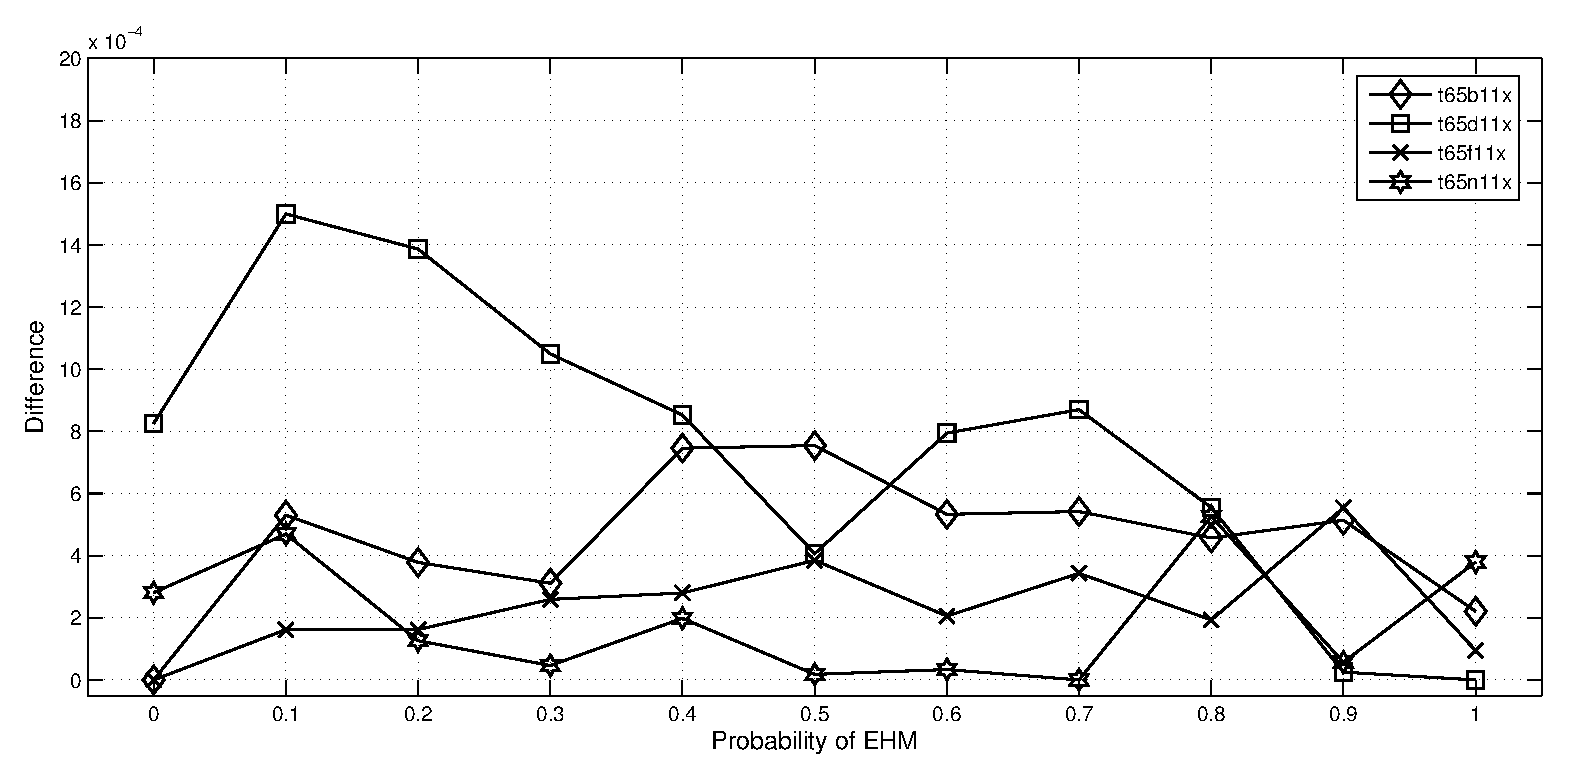
\includegraphics[width=1.0\textwidth]{img/sweep_lop.eps}
        % \caption{LOP}
    % \end{subfigure}\\
    % \begin{subfigure}{1.0\textwidth}
        % 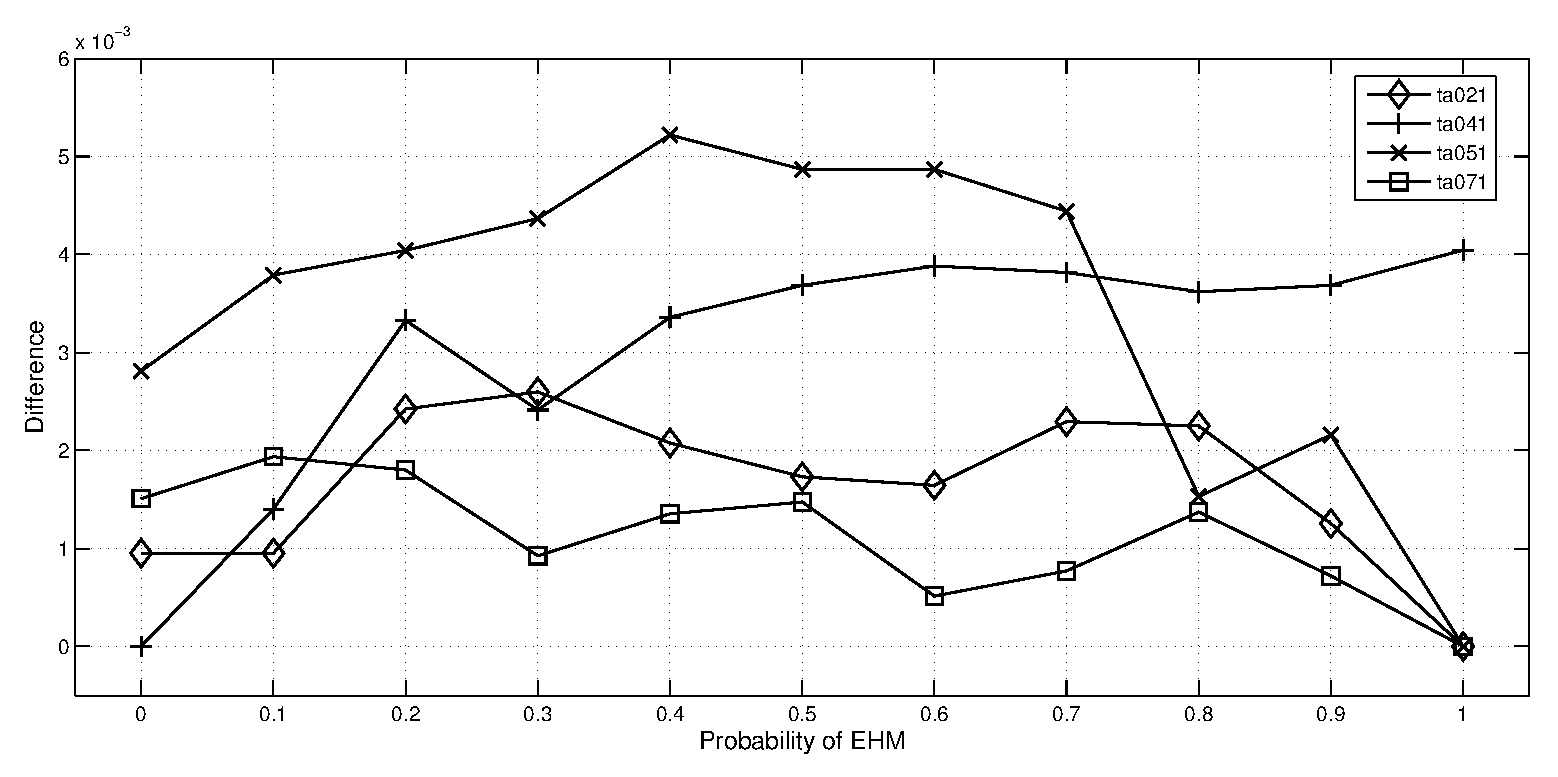
\includegraphics[width=1.0\textwidth]{img/sweep_pfsp.eps}
        % \caption{PFSP}
    % \end{subfigure}
    % \caption{Difference of average of each probability $p$ }
    % \label{fig:sweep}
% \end{figure}

\begin{figure}[t]
    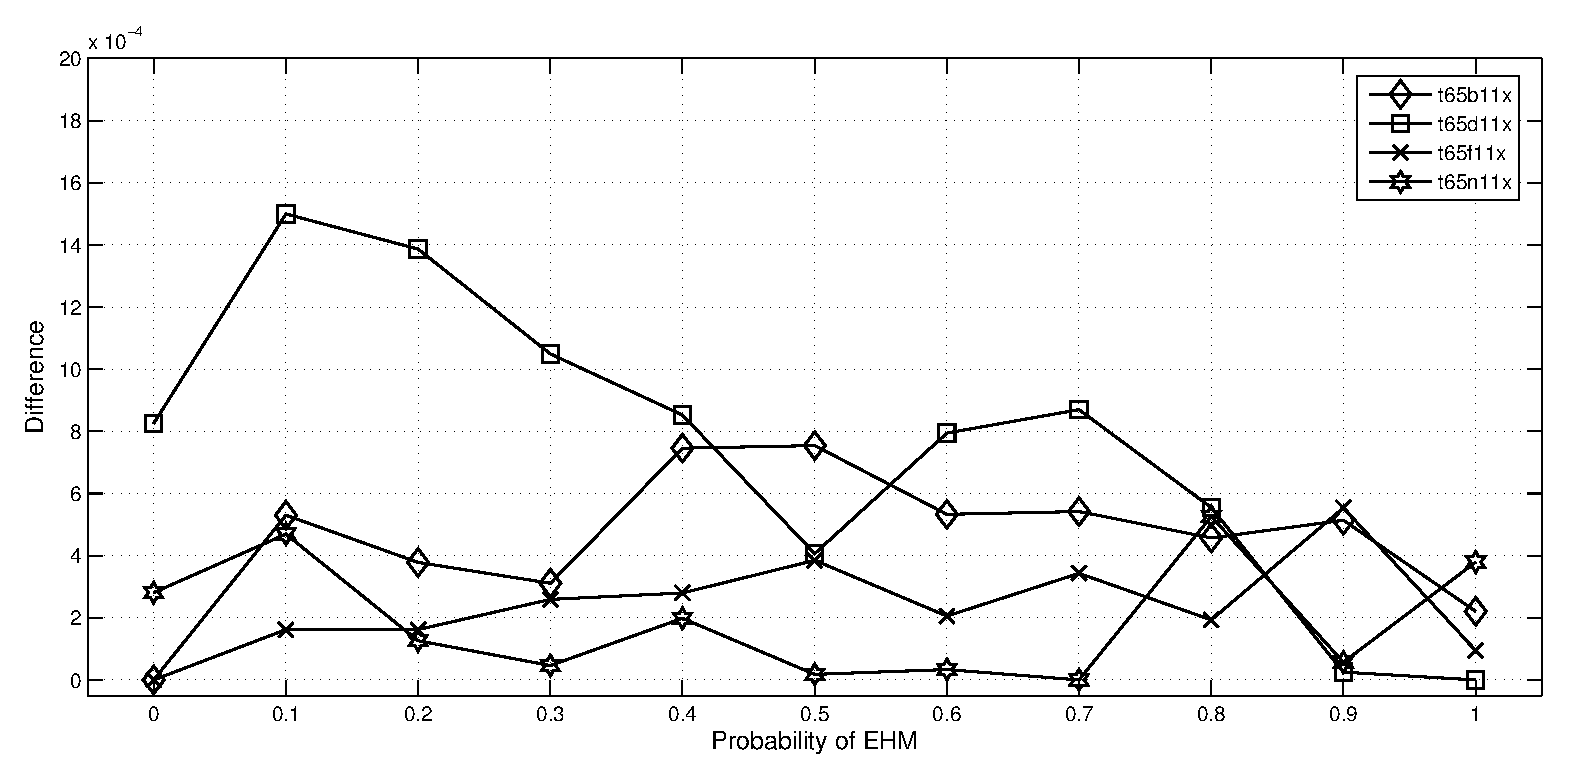
\includegraphics[width=1.0\textwidth]{img/sweep_lop.eps}

    \caption{Difference of average of each probability $p$ on LOP}
    \label{fig:sweep_lop}
\end{figure}









Figures \ref{fig:sweep_lop} shows the difference between average of each probability. The values on the $y$-axis is the normalized difference between the average the best objective values in each trial and the worst average of object values among all trials. The higher the values is, the better the performance. The values on the $x$-axis are the probability $p$ of to sampling EHM. In other word, the value $p=1.0$ indicates that the hybrid algorithm is identical to EHBSA which is by pure EHM, and the value $p=0.0$ indicates that the hybrid algorithm is identical to NHBSA which is by pure NHM.

As can be seen, in some instances of PFSP, the best objective value is obtained in the trials that both models have chance to sample new individual. In all of the instances of LOP, the experiments with only one model have lower object value than the one with hybridization of two models. These experiments indicate that mixing different models can be more efficient when solving permutation problems. Thus, we make the three attempt at model adaptation in the follow chapters.


% \subsection{Summary}
% In this chapter, the model-choosing experiment shows the impact of inappropriate model. Since the model-choosing significantly effects the performance of the EDAs for permutation problem, the semantics of problems must be studied for better performance. But the semantics of real-life problems is not always trivial as TSP and QAP. It makes finding a appropriate model a difficult task. Next, the second experiment uses the sweep method to investigate the improvement possibility of incorporating multi-models. The result shows that incorporating multi-models can achieve better performance on problems like PFSP and LOP which models cannot precisely describe.

\section{The Enumeration Method}

At the first attempt, we use enumeration method to choose model. This chapter shows the algorithm of enumeration method. Besides, we test enumeration method on different permutation problems, and this experiments shows advantages and disadvantages of enumeration method.

For the highest fitness solution, every type of problems needs a most expressive semantic model to express. Although the literature has deep knowledge about some of permutation problems, new problems are still formatted into permutation problems consistently, to which the existing models cannot precisely capture. When the semantics is beyond the capability of existing models, another new expressive  semantic model for the specific problem from new problems is needed. Unfortunately, designing new semantic models is not a trivial work. In the second experiment of the previous section, the result shows the potential of mixing different models. The experiment also shows that with limited semantic models, through incorporating different semantic models, the hybridization of EHM and NHM solve the specific problems without the expressive semantic model more efficiently than algorithms with single model. Although we can find the best parameter setting through sweeping each mixing ratio thoroughly, it is impractical when the number of used semantic models grows.


{\LinesNumbered
\begin{algorithm}[htbp]
     \KwIn{The initial population $P$,\newline
    The semantic model set $\mathbb{M}$
    }
    \KwOut{The offspring population $O$}

        build every semantic model for $P$\;
        
        randomly chose $p \in P$\ as template\; 
        initialize an individual set $C$ \;
        \For {$m \in \mathbb{M} $ }{
        generate a new individual c by model $m$\;
        $C \leftarrow C\cup\lbrace c \rbrace$$ \;
        }
        $c$ \leftarrow the best solution $\in C$\;
        $O$ \leftarrow $P \cup \{c\} - \{p\}$\;
        return $O$\;
    \caption{The Enumeration Model}
    \label{alg:enumeration_method}
\end{algorithm}}

In the enumeration method, multiple semantic models generate new solution candidates, and the best one is chosen. This chapter shows that the strategy of generating new individuals from multiple models at once and keeping the best descendant in population outperform in some problems. 

The enumeration method acts almost similarly to EHBSA or NHBSA except for multiple models. In each generation, the enumeration method randomly picks one individual from the population as template and then generates new individuals from each models with the picked template if need. Next, the population keeps the best individual among the newly generated individuals and the template, and discards the rest. Finally, the enumeration updates each semantic models with the new population, and continues the evolution until the terminal criterion is met. The pseudo-code is in Algorithm \ref{alg:enumeration_method}. 


In our experiments, we perform enumeration method with the population size $N = 2 \times L$ and the NFE limit $E_{max} = L \times 40000$. And template technique is used, NHM and EHM are used semantic models. The cut-point number is 3 for template.

%In the experiments of the enumeration method, the EHM and the NHM %are used. The experiment settings are as follows:
%\begin{itemize}
    %\item repeat 10 times,
   % \item the NHM and the EHM are used,
   % \item population size $N = 2 \times L$ ($L$ is the problem size),
   % \item the bias ratio $B_{ratio} = 0.0000$,
   % \item the NFE $E_{max} = L \times 40000$,
   % \item template technique is used,
   % \item the cut-point number is 3 for template.
%\end{itemize}

\begin{table}[t]
    \centering
    \begin{tabular}{|l|l|l|l|l|l|l|l|}
    \hline
    \textbf{}         & \textbf{EHBSA}    & \textbf{Enum2} & \textbf{NHBSA} & \textbf{}         & \textbf{EHBSA}    & \textbf{Enum2} & \textbf{NHBSA} \\ \hline
    \multicolumn{4}{|c|}{\textbf{LOP}}                              & \multicolumn{4}{c|}{\textbf{TSP}}                                \\ \hline
    \textbf{t65b11xx} & 1              & 2              & 3         & \textbf{burma14}   & 2              & 2              & 2         \\ \hline
    \textbf{t65d11xx} & 3              & 1              & 2         & \textbf{bayg29}    & 2              & 3              & 1         \\ \hline
    \textbf{t65f11xx} & 2              & 1              & 3         & \textbf{dantzig42} & 2              & 3              & 1         \\ \hline
    \textbf{t65n11xx} & 2              & 1              & 3         & \textbf{eil51}     & 1              & 3              & 2         \\ \hline
    \textbf{t65w11xx} & 3              & 1              & 2         & \textbf{berlin52}  & 2              & 3              & 1         \\ \hline
    \textbf{t69r11xx} & 2              & 1              & 3         & \textbf{eil76}     & 1              & 3              & 2         \\ \hline
    \textbf{t75i11xx} & 3              & 2              & 1         & \textbf{eil101}    & 1              & 3              & 2         \\ \hline
    \multicolumn{4}{|c|}{\textbf{PFSP}}                                      & \multicolumn{4}{c|}{\textbf{QAP}}                                         \\ \hline
    \textbf{ta001}    & 1              & 2              & 3         & \textbf{nug17}     & 3              & 1              & 2         \\ \hline
    \textbf{ta021}    & 3              & 1              & 2         & \textbf{nug18}     & 3              & 2              & 1         \\ \hline
    \textbf{ta031}    & 1.5            & 1.5            & 3         & \textbf{nug20}     & 3              & 2              & 1         \\ \hline
    \textbf{ta041}    & 2              & 1              & 3         & \textbf{nug21}     & 3              & 2              & 1         \\ \hline
    \textbf{ta051}    & 3              & 1              & 2         & \textbf{tai10a}    & 2              & 3              & 1         \\ \hline
    \textbf{ta061}    & 1.5            & 1.5            & 3         & \textbf{bur26a}    & 3              & 2              & 1         \\ \hline
    \textbf{ta071}    & 2              & 1              & 3         & \textbf{bur26b}    & 3              & 2              & 1         \\ \hline
    \end{tabular}

\caption{Rank of algorithms, comparison for the 2-model enumeration method}
\label{tb:enumeration_case1}
\end{table}



The results are in Table \ref{tb:enumeration_case1}. Four problems are tested in the experiment. In our experiments, we use the fractional ranking system as the index of the performance. Then rank is sorted by the average fitness of each algorithm. The lower the rank is, the better the performance. Items that compare equal receive the same ranking number, which is the mean of what they would have under ordinal rankings. Equivalently, the ranking number of 1 plus the number of items ranked above it plus half the number of items equal to it. This strategy has the property that the sum of the ranking numbers is the same as under ordinal ranking. Table \ref{tb:enumeration_case1} shows that the enumeration outperformed the other algorithms on LOP and PFSP. On the contrary, the enumeration method underperformed on TSP and QAP. In this experiments, the enumeration method performs better on the problems without a existing expressive semantic model for the specific problem from the problems.


In spite of the higher fitness solution on the problems without a existing expressive semantic model for the specific problem from the problems, the enumeration method shows worse performance on problems which have the expressive semantic models for the problems. Furthermore, adding new models into the system makes the situation even worse. Since the enumeration method iterates all of models in system, it wastes lots of resources on unexpressive models, instead of only focusing on the models which can generating competitive solutions. Thus, we attempt to develop another method in the follow chapter.

% \begin{table}
% \label{fig:enumeration_case2}
% \caption{The Three Model Enumeration Method}
% \end{table}


% For scaling up and generalizing the enumeration method, the second experiment investigates the performance of adding the third model, the Plackett-Luce ranking model. The experiment setting remains the same as the first experiment ,besides the Plackett-Luce model is used. In second experiment, the Plackett-Luce model follows the evolutionary framework proposed by Tsutsui~\citep{tsutsui2002probabilistic}, instead of the original framework proposed by Ceberio \emph{et~al.} in~\citep{ceberio2013plackett}, to compare the algorithms purely evolving with semantic models. 

% The result of second experiment is listed in Figure \ref{fig:enumeration_case2}. Although the enumeration method outperformed the other algorithms on PFSP, the other algorithms outperformed the enumeration method on the three other problems. On LOP, the Plackett-Luce model outperforms the enumeration model, because it can describes the relative ordering semantics well. 

% Remarkably, after the Plackett-Luce model was added into the system, the overall performance of each problems reduces. The performance difference is shown in Table \ref{}.  
\section{The Bayesian Method}
At the second attempt, we use Bayesian probability to determine which semantic model is chosen. This chapter shows the introduction of Bayesian probability, the method of model adaptation. Besides, we investigate the issue of this method.

To avoid wasting lots of resources on unexpressive models, we need a more advanced model adaptation technique. That is to say, the model adaptation should invest the limited computing resources in the promising model more often and explore different models when the most expressive model is uncertain. For this purpose, the probability of choosing the model is measured in terms of the Bayesian posterior probability.

Although this method can work theoretically, it doesn't work as expected in our experiments. We will describe this phenomenon in the follow section.

 
\subsection{The Bayesian Posterior Probability}
In Bayesian inferencing, the posterior probability~\citep{lee2012bayesian} of a random event is the conditional probability that is assigned after the relevant evidence is taken into consideration. Similarly, the posterior probability distribution is the probability distribution of an unknown quantity, treated as a random variable, conditional on the evidence got from an experiment.

%The posterior probability is the probability of the parameter $\theta$ given the evidence $X:P(\theta|x)$. It contrasts with the likelihood function, which is the probability of the evidence given the parameters: $p(x|\theta)$. Let us have a prior belief that the probability distribution function is $p(\theta)$ and observation $x$ with the likelihood $p(x|\theta)$, and then the posterior probability is defined as
%\begin{equation}
%p(\theta|x) = \frac{p(x|\theta)p(\theta)}{p(x)}
%\end{equation}.

In our case, we want to measure the posterior probability of a semantic model given the permutation problem $P$: $Pr(M|P)$. Assuming all semantic models are equally probable, the posterior is proportional to its likelihood $Pr(P | M)$, which can be easily calculated as $ Pr(P | M) =
    \prod_{\forall i \in P}{Pr(i|M)}\text{,}$ 
where $P$ is the population containing individuals and $Pr(i|M)$ is the conditional probability of a specific individual in the population given the semantic model. 



\subsection{Model Adaptation}
{\LinesNumbered
\begin{algorithm}[htbp]
     \KwIn{The initial population $P$,\newline
    The semantic model set $\mathbb{M}$
    }
    \KwOut{The offspring population $O$}


        build each semantic model $m \in \mathbb{M}$ for $P$\;
        measure the posterior of each model $m \in \mathbb{M}$ according to $P$\;
        offspring population $O := \{\}$\;
        \ForEach{$p \in P$}{
            choose a model $m$ according the probability distribution $P(\mathbb{M})$\;
            let $p$ be the template, generate a new individual $c$ by model $m$\;
            \If{$c$ is better than $p$}{ $O$ := $O \cup \{c\}$\; } 
            \Else{$O$ := $O \cup \{p\}$\; }

        }
        return $O$\;
    \caption{The Bayesian Method}
    \label{alg:bayesian_method}
\end{algorithm}}
Since we have the method to measure the posterior of the semantic models, this method can be applied to the model adaptation. For the preliminary study, the posterior of the semantic model is directly used as the probability of choosing the model to generate new individuals.

Formally, for each model $m \in M$, where $M$ is the set of the models the system has, $Pr(m)$ is the probability that the model $m$ is chosen as the most expressive model to generate new individuals among the model set $M$. The probability is defined as
\begin{equation*}
    Pr(m) = \frac{q_m}{\Sigma_{j \in M} {q_j} }\text{,}
\end{equation*}
where $q_j$ is the posterior of the semantic model $j$. 

For model adaptation, the Bayesian method chooses a model before the sampling phase. Because the population reflect the semantics of the permutations as the population evolves, the posterior of the expressive models for the specific permutation problem increases. Hence, these models for the specific permutation problem have more chance to generate new individuals, while the other candidate models still have little chance.

The pseudo code is in Algorithm \ref{alg:bayesian_method}. The model adaptation stage between model building and sampling. Let the population size be $N$. In every generation, the Bayesian method  iterates the whole population to make each individual template for generating new individual, and then keeps the better one between new generated offspring and the template. This difference accelerates the population reflecting the problem semantics, due to the population moves toward the high fitness solutions.  


\subsection{Empirical Study}
In this subsection, the performance of the Bayesian method is investigated. In practice, the conditional probability of the population given the model will be expressed in logarithm for computation convenience, since the value is too small for the float-point number in computer. 

For the experiment purpose,  TSP and the flat problem are tested. The objective value of the flat problem is a constant, no matter the permutation is. Hence, the posterior of the solution on the flat problem is independent from the semantic models. 

\begin{figure}[t]     
    \begin{subfigure}{1.0\textwidth}
        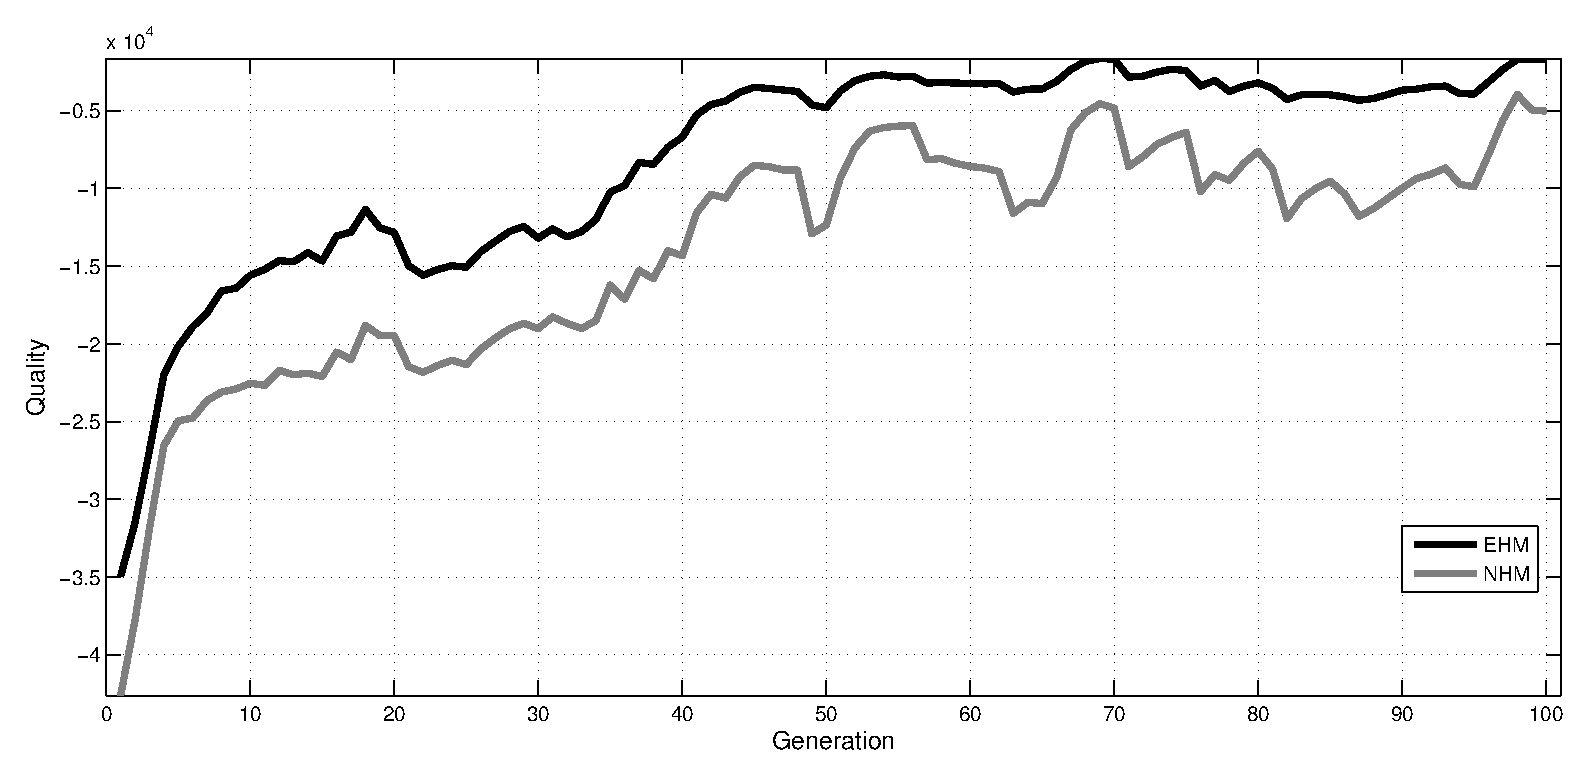
\includegraphics[width=1.0\textwidth]{bayesian_tsp.eps}
        \caption{TSP, eil51, $L=51$, $N=1000$}
    \end{subfigure}\\

    \begin{subfigure}{1.0\textwidth}
        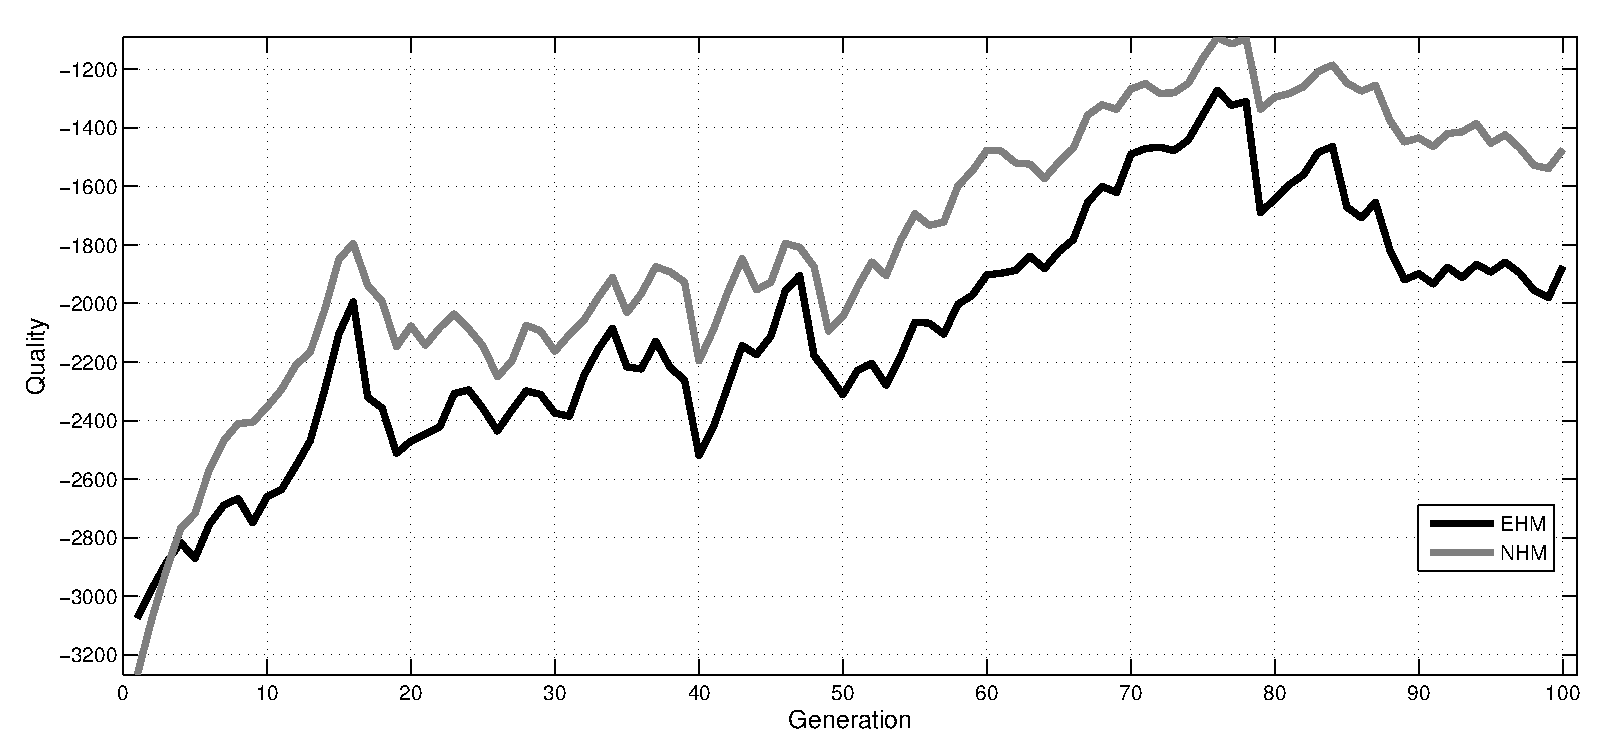
\includegraphics[width=1.0\textwidth]{bayesian_flat.eps}
        \caption{Flat, $L=50$, $N=100$}
    \end{subfigure}
    \caption{(Temp)The posterior of the semantic model, tournament selection $S=2$ }
    \label{fig:bayesian_quality}
\end{figure}

In the experiment of the Bayesian method, EHM and NHM are used. The population size $N$ is $1000$ for TSP and $N$ is 100 for the flat problem. We perform independent 10 runs on each instance. The problem size of the flat problem is $50$. The instance eil51 of TSP has been used in this empirical study \footnote{\textbf{TSPLIB} http://www.iwr.uni-heidelberg.de/groups/comopt/software/TSPLIB95/}.%The experiment settings are as the follows:
%\begin{itemize}
    %\item repeat 10 times,
   % \item the NHM and the EHM are used,
   % \item population size $N=1000$ for TSP and $N=100$ for the flat problem,
   % \item the bias ratio $B_{ratio} = 0.0000$,
   % \item template technique is used,
   % \item the cut-point number is 3 for template.
%\end{itemize}
 

Figure \ref{fig:bayesian_quality} shows the posterior of the semantic models in term of the logarithm the conditional probability of the population given the semantic model. The higher the posterior, the better the model describes the problem. As can be seen, at the beginning of the trials on the flat problem and TSP, the posterior of NHM is lower than that of EHM. After 5 generations, the posterior of NHM becomes higher than that of EHM on the flat problem and remains higher until the trial ends. 

Although the posterior of EHM in TSP is higher than that of NHM as we expected, the posterior of NHM on TSP grows faster than EHM as the population evolves. To demonstrate the phenomenon, we test the flat problem in our experiments. The posterior of the both models on the flat problem is not identical as we expected. This result shows that NHM is more sensitive than EHM to population changes.

Of course, these effects of the phenomenon can be eliminated by preproduce. However, introducing new techniques to the Bayesian method for balancing different models also increase the cost of adding new models into this system, so we attempt to develop another method in the follow chapter.


% Since the semantics of permutation problem differs, many dedicated models are designed for specific permutation problems. For example, the EHBSA outperforms than other algorithms on TSP~\citep{tsutsui2002probabilistic}, while the NHBSA is dedicated to the problems with strong relation of absolute positions of indices like QAP. Despite the diversity of semantics, a model can only focus on specific permutation problems. Furthermore, The semantics of permutation is not always clear to the literature. It increases the difficulty to chooses the appropriate model to solve the permutation problems. As a result, existing models can not perfectly capture the core semantics which beyond the capability of existing models. 

% To conquer the difficulty of EDAs on permutation problems, a tool allowing EDAs to adapt itself to the problems is needed. The model adaptation framework should determine which semantic model is the fittest for the problem and acquire the solutions as close as possible to the global optima. To Achieve this, learning techniques are necessary for the model adaptation. Similarly, the model adaptation also faces the some difficulty when choosing model to sample new individual. When the system initials, no prior knowledge about the relation between the problem and the models is given. Through repeated trials within limited NFE, the system has to find out the fittest model for specific problem and manages to yield the solution as close as possible to the result a single model EDA would provide.




\section{Multi-armed Bandit Based Model Adaptation}
At the last attempt, we use the UCB algorithm to choose model. The UCB algorithm is commonly used to solve multi-armed bandit problem. This chapter shows the introduction of UCB and the model adaptation framework.

Ideally, we choose one of the most expressive semantic models for the problem in each generation to reduce NFE. However, without given the semantics of the problem in prior, we can only explore several different semantic models information before fully exploiting the most promising model. Therefore, we use the techniques from the multi-armed bandit problem to balance exploration and exploitation.

\subsection{Multi-armed Bandit Problem}
% Multi-Armed Bandit Algorithms and Empirical Evaluation
A multi-armed bandit (MAB) is like a traditional slot machine but with $K$ levers. When pulled, each lever provides a reward drawn from the distribution associated to that specific lever. The gambler has no prior knowledge of reward distribution of the levers, but through repeated trials, he can focus on the most profitable lever~\citep{Mohri2005, Kuleshov2000}.

The classic MAB problem consists of random variables $X_{i,n}$ for $1\leq i\leq K$ and $n\geq 1$, where each $i$ stands for the index of a gambling machine (\textit{i.e.}, the arm of a bandit). Successive plays of machine $i$ yield rewards $X_{i,1}, X_{i,2},...$ which are independent and identically distributed by unknown law and with unknown expectation. 

For a formal definition, the random variables are independent across the arms and are associated to probability distributions $(D_1, D_2,...,D_k)$ with  expectations $(\mu_1, \mu_2,...,\mu_k)$ and variances $(\sigma_1, \sigma_2,...,\sigma_k)$. Throughout the playing, the distributions are unknown for gambler. The goal for gambler is to collect as much rewards as possible by pulling the armed over many times. At each turn, $t=1,2,...$, the gambler selects an arm, with index $j(t)$ and the times played $n$, and receives a reward $X_{j(t),n}$. The MAB algorithms specify a strategy or a polity by
which the gambler should choose an arm $i$ at each turn. 

%  Asymptotically efficient adaptive allocation rules.
The most popular performance measure for bandit algorithms is the total \textit{expected regret},
defined for any fixed turn $T$ as:
\begin{equation*}
    R_T = T\mu^* - \sum^T_{t=1}{\mu_{j(t)}} \text{,}
\end{equation*}
where $\mu^* = \max_{i=1,...,k}{\mu_i}$ is the expected reward from the best arm.  Thus, the regret is the loss caused by the policy not always playing the best machine. For a large class of pay-off distributions, there is no policy whose regret would grow slower than $O(\ln n)$~\citep{lai1985asymptotically}. For such pay-off distributions, a policy is said to resolve the exploration-exploitation trade-off if its regret growth rate is within a constant factor of the best possible regret rate.


\subsection*{Upper Confidence Bound Algorithms}
% 2002 - Finite-time Analysis of the Multi-armed Bandit Problem
% 2006 - Bandit Based Monte-Carlo Planning
The UCB algorithms have been proposed by~\citep{Auer2002, Auer2002ucb} which are a family of widely used in the MAB problem.  The UCB family was designed as a simpler, more elegant implementation of the idea of optimism in the face of uncertainty, proposed by Lai \& Robbins~\citep{lai1985asymptotically}. An extension of UCB-style algorithms to sequential, tree-based planning was developed in~\citep{Kocsis2006}, and it has been proved very successful in Go playing programs~\citep{Kocsis2006, Gelly2007, Gelly2008}.  

Algorithm UCB1, whose finite-time regret is studied in details by~\citep{Auer2002}, is a simplest algorithm that succeeds in resolving the exploration-exploitation trade-off. In the UCB, rewards are either 0 or 1, and the empirical quality $\overline{x}$ lies in $[0,1]$. It keeps track the average rewards $X_i, T_i(t - 1)$ for all the arms and chooses the arm with the best upper confidence bound:
\begin{equation}
	I_t = \argmax_{i\in \{1,...,K\}}{\overline{X}_{i,T_i(t-1)}+c_{t-1,T_i(t-1)}},
\end{equation}
where $c_{t,s}$ is a bias sequence chosen to be
\begin{equation}
	C_{t,s}=\sqrt{\frac{2\ln t}{s}}.
\end{equation}
The bias sequence is such that if $X_{it}$ were independently and identically distributed then the inequalities
\begin{equation}
\left\{\begin{matrix}
    \mathbb{P}(\overline{X}\geq \mu_i+c_{t,s})\leq t^{-4},\\ 
    \mathbb{P}(\overline{X}\leq \mu_i-c_{t,s})\leq t^{-4}
\end{matrix}\right.\text{}
\end{equation}
were satisfied. This follows from Hoeffding's inequality.

The authors also propose another algorithm, UCB1-Tuned, which they claim performs better in practice but comes without theoretical guarantees. The main feature of UCB1-Tuned is that it takes into account the variance of each arm and not only its empirical mean. More specifically, at turn $t = 1, 2,...$ the algorithm picks an arm $j(t)$ as 
\begin{equation}
   j(t) = \argmax_{i\in \{1,...,K\}}{\left(\mu_i + \sqrt{ \frac{\ln t}{n_i}\min{\left(\frac{1}{4}, V_i(n_i)\right)}  } \right)},
\end{equation}
where
\begin{equation}
   V_i(t) = \sigma_i^2(t) + \sqrt{\frac{2\ln t}{n_i(t)}}.
\end{equation}

The estimate of the variance $\sigma_i^2(t)$ can be computed as usual by maintaining the empirical sum of squares of the reward, in addition to the empirical mean. Audibert \textit{et al.}~\citep{audibert2009exploration} provide expected regret bounds and regret concentration results for variance-based UCB algorithms similar to UCB1-Tuned.



\subsection{The Proposed Framework}
\begin{figure}[t]
    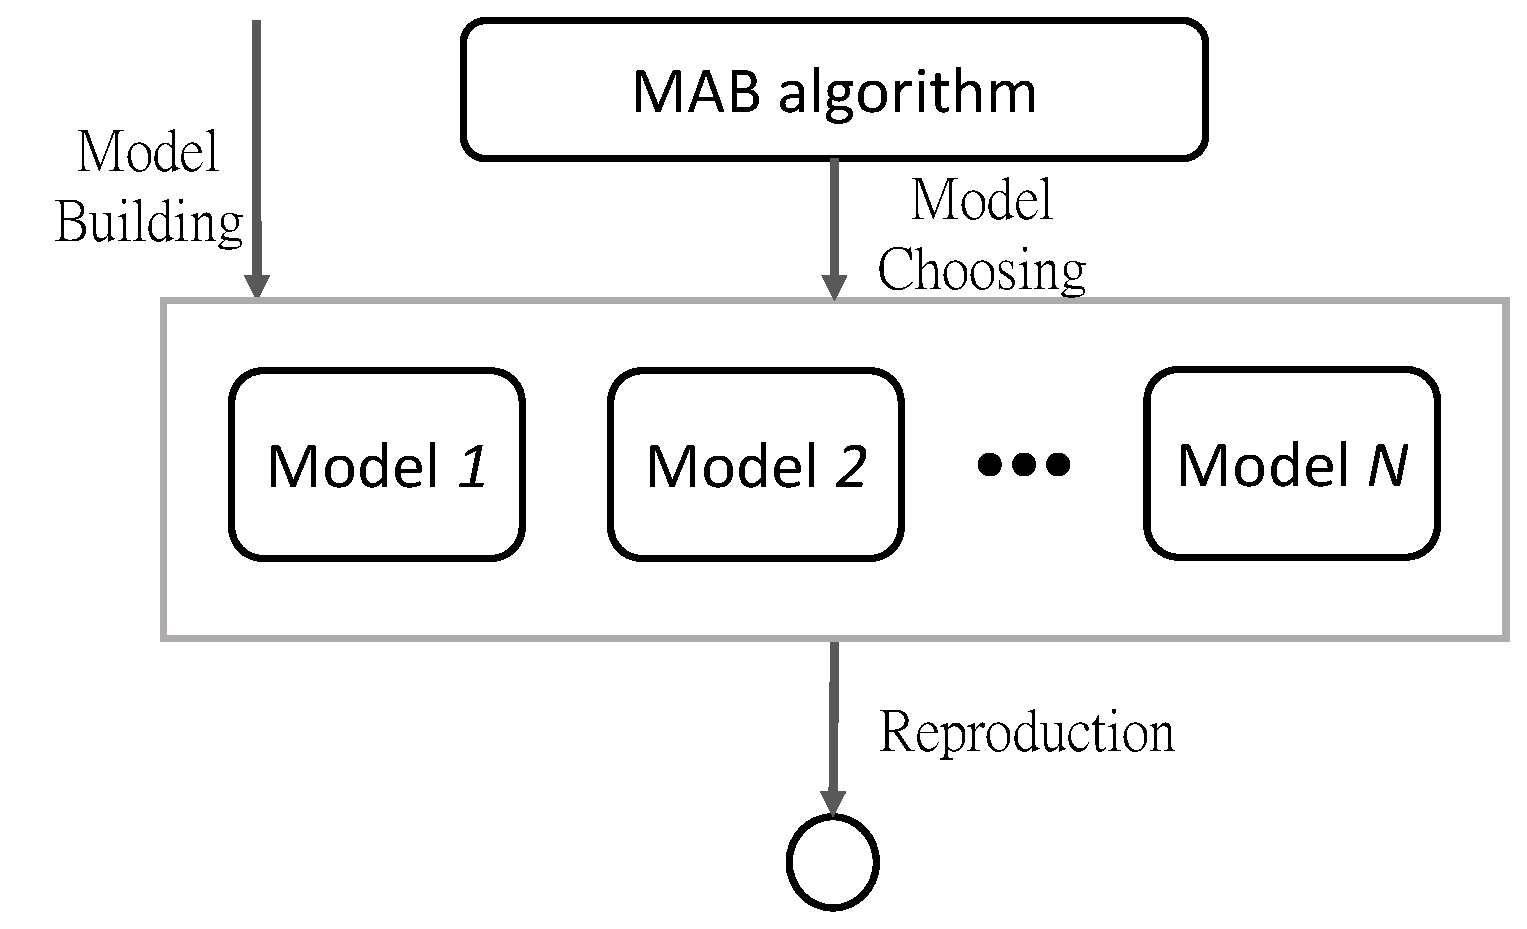
\includegraphics[width=0.8\textwidth]{model_adaptation_flow.eps}
    \caption{The Model Adaptation Flow}
    \label{fig:model_adaptation_flow}
\end{figure}
In this paper, the model adaptation framework incorporates with the UCB algorithms for a preliminary study. Although many other MAB techniques exist and show good performances~\citep{Kuleshov2000}, the UCB family is commonly used recent years, and is easy to be implemented. Figure \ref{fig:model_adaptation_flow} shows the flow of the model adaptation framework. Along with the original EDA framework, the model adaptation adds a new phase ``Model Choosing'' between phase ``Model Building'' and ``Sampling''. As can be seen, instead of generating a population of new individual with one model in the original version of sampling procedure, in our framework, new individuals are sampled one by one with different models. 
{\LinesNumbered
\begin{algorithm}[htbp]
\SetKwInOut{Input}{input}
    \SetKwInOut{Output}{output}

    \KwIn{The initial population $P$,\newline
    The semantic model set $\mathbb{M}$
    }
    \KwOut{The offspring population $O$}
        generate one individuals from each model\;
        
            %select population of promising solution $S$\;
            update each model $m \in \mathbb{M}$\;
                randomly chose $p \in P$\;
                choose a semantic model $m_{UCB}$ with \textit{highest UCB value}\;
                
                let $p$ be the template, generate a new individual $c$ by model $m_{UCB}$\;
                \If{$c$ is better than $p$}{ 
                    $O \leftarrow P \cup \{c\} - \{p\}$\; 
                    reward model $m_j$ with value $1.0$\;
                } 
                \Else{
                    $O \leftarrow P$; \newline 
                    reward model $m_j$ with value $0.0$\;
                }
                
   
        return $O$\;
    \caption{Multi-armed Bandit Based Model Adaptation}
    \label{alg:model_adaptation}
\end{algorithm}}


Algorithm \ref{alg:model_adaptation} introduces a details pseudo-code of the proposed multi-armed bandit based model adaptation (MABMA). Lines 10 and 11 replace $p$ with the newly generated individual $c$. To improve performance, we will introduce a new methodology to choose replaced individual in next chapter. As we treat the semantic models as arms in the MAB problem, at the initialization stage of the algorithm, the UCB algorithms needs initial value of the semantic models. Thus, each model $m_j$ have to generate one new individual by a randomly picked template for the initialization of UCB.

% Toward Comparison-based Adaptive Operator Selection
Properly rewarding the selected arm is a crucial element that should be carefully designed to ensure success~\citep{fialho2010analyzing}. The choice of the reward must encourage exploitation of the best arm while still allowing exploration of the other arms. Most methods use as raw reward the fitness improvement of the newborn offspring compared to a base individual, that might be its parent~\citep{barbosa2000adaptive, fialho2008extreme, fialho2009analysis, lobo1997decision, tuson1998adapting}, the current best in the population~\citep{Davis:1989:AOP:93126.93146}, or the median individual of the current population~\citep{Julstrom:1995:YDM:645514.657934}. The concept used in our case is borrowed from an assumption made in original UCB~\citep{Auer2002} -- the reward are with support in $[0,1]$. The reward given to the bandit is binary. An arm is assigned a reward of $1$ if the fitness of the newborn individual is better than the template, and 0 otherwise. 

%Sustainable Cooperative Coevolution with a Multi-Armed Bandit
This reward policy shares similar arguments with the policy used in~\citep{DeRainville:2013:SCC:2463372.2463556}. The direct fitness allocation suffers when the bandit is updated with a new fitness causing a loss -- if this fitness dominates any other arm causing a gain, the arm receives a higher credit for the loss. Since the template plays a critical role in the fitness of the new born individual, the fitness cannot reflect the appropriateness of a semantic model. Furthermore, the scale of the fitness value dramatically differs from problem to problem, or even from instance to instance. The fitness can not reflect the difference between two permutations. For instance, two permutation could have huge difference in the fitness because merely two nodes swapped its position in the permutation.


\subsection{Empirical Study}

In this subsection, the performance of MABMA is investigated. Several permutation problems are tested. For comparison, MABMA with  UCB1 and UCB1-Tuned are be tested. In the experiment of Multi-armed Bandit Based Model Adaptation,  EHM, NHM and the PL model are used. For each instance, we perform independent 10 runs with the population size $N = 2 \times L$ and the NFE limit $E_{max} = L \times 40000$. In this section, CVRP and the variation of CVRP -- the vehicle routing problem with Time Window (VRPTW)~\citep{toth2001vehicle} -- are tested.

%The experiment settings are as follows:
%\begin{itemize}
    %\item repeat 10 times,
    %\item the NHM, the EHM  and the PL model are used,
    %\item population size $N=1000$ for TSP and $N=100$ for the flat problem,
    %\item the bias ratio $B_{ratio} = 0.0000$,
    %\item template technique is used,
    %\item the cut-point number is 3 for template.
%\end{itemize}

\begin{table}[t]
    \centering
    \begin{tabular}{|l|l|l|l|l|l|}
    \hline
    \textbf{} & \textbf{EHBSA}       & \textbf{MABMA-UCB1} & \textbf{MABMA-UCBT} & \textbf{NHBSA} & \textbf{PLEDA} \\ \hline
    \textbf{A-n32-k5} & 1            & 5                  & 3              & 2           & 4         \\ \hline
    \textbf{A-n33-k5} & 1.5          & 4                  & 1.5            & 3           & 5         \\ \hline
    \textbf{A-n33-k6} & 1.5          & 1.5                & 3              & 4           & 5         \\ \hline
    \textbf{A-n34-k5} & 1            & 2                  & 3              & 4           & 5         \\ \hline
    \textbf{A-n36-k5} & 1            & 4                  & 2              & 3           & 5         \\ \hline
    \textbf{A-n63-k9} & 2            & 3                  & 1              & 4           & 5         \\ \hline
    \textbf{A-n64-k9} & 1            & 2                  & 3              & 4           & 5         \\ \hline
    \textbf{A-n65-k9} & 1            & 2                  & 3              & 4           & 5         \\ \hline
    \textbf{A-n69-k9} & 1            & 3                  & 2              & 4           & 5         \\ \hline
    \textbf{A-n80-k9} & 1            & 3                  & 2              & 4           & 5         \\ \hline
    \end{tabular} 
    \caption{The rank on CVRP}
    \label{tb:mabma_result}
\end{table}

\begin{table}[t]
    \centering
        \begin{tabular}{|l|l|l|l|l|l|}
        \hline
        \textbf{} & \textbf{EHBSA}       & \textbf{MABMA-UCB1} & \textbf{MABMA-UCBT} & \textbf{NHBSA} & \textbf{PLEDA} \\ \hline
        \textbf{C101\_0025}  & 2                  & 2                   & 2              & 4           & 5         \\ \hline
        \textbf{C103\_0025}  & 2                  & 2                   & 2              & 4           & 5         \\ \hline
        \textbf{RC102\_0025} & 1                  & 2                   & 3              & 5           & 4         \\ \hline
        \textbf{RC105\_0050} & 3                  & 2                   & 1              & 4           & 5         \\ \hline
        \textbf{C101\_0100}  & 4                  & 1                   & 2              & 3           & 5         \\ \hline
        \textbf{C101\_0025}  & 3                  & 1.5                 & 1.5            & 4           & 5         \\ \hline
        \textbf{C103\_0025}  & 3                  & 1.5                 & 1.5            & 4           & 5         \\ \hline
        \textbf{RC102\_0025} & 1                  & 2                   & 3              & 5           & 4         \\ \hline
        \textbf{RC105\_0050} & 3                  & 2                   & 1              & 4           & 5         \\ \hline
        \textbf{C101\_0100}  & 4                  & 1                   & 2              & 3           & 5         \\ \hline
        \end{tabular}
    \caption{The rank of the fvVRPTW}
    \label{tb:mabma_result}
\end{table}

    


The results are shown in Table \ref{tb:mabma_result}. MABMA-UCB1 is for MABMA with the UCB1 algorithm; MABMA-UCBT is for MABMA with the UCB1-Tuned algorithm. The values listed in the tables are the average of the best fitness of the algorithm obtained in 10 trials. Because CVRP aims to minimize the distance vehicles traveled, the fitness is the smaller, the better the performance. 

In CVRP instances, EHBSA outperforms the other algorithms. As can be seen, the average fitnesses of the MABMA algorithms are most close to the ones of optimal model, EHM. As the problem size becomes larger, the difference between EHBSA and MABMA decreases. In the fvVRPTW, MABMAs outperform the other algorithms on large problem instances. On the easier problem instance, MABMAs and EHBSA has identically performance, because they achieve the optimal solution.

Remarkably, on CVRP, the performance of MABMA-UCBT is more closer to that of EHBSA than that of MABMA-UCB1, while MABMA-UCB1 achieve better performance in the fvVRPTW. This fact may be caused by the variance factor in the UCB1-Tuned algorithm can help the MABMA stick to the most appropriate model better. However, when the most appropriate model is not existed, the UCB1 algorithm can start to explore in the earlier stage.



%\section{Replacement Strategy}
\label{ch:replacement_strategy}

In the previous section, we introduce three semantics of permutation problems, three existing semantic models, MABMA. This section focuses on replacement strategy, give a brief introduction to the restricted tournament replacement (RTR) and incorporates these into the whole. This section defines three distance measures of RTR: edge distance, node distance and order distance, shows the effects of RTR on permutation problems and the essence of distance-measure choosing, proposes a method for choosing distance measure of RTR, improves reward policy of model adaptation, gives suggested setting of window size of RTR for permutation problems and shows the difference between original MABMA and MABMA with distance-measure choosing.




\subsection{Restricted Tournament Replacement}
The restricted tournament replacement (RTR) is a commonly used niching technique in the field of EDAs. RTR is also known as restricted tournament selection (RTS) which is first proposed in \citep{Harik1995}. RTR uses the tournament strategy to decide the part which get to move on to the next generation. We present the process of RTR in algorithm \ref{alg:RTR_algorithm}, where the $Distance$ function is usually the Hamming distance in binary problems. However, Hamming distance is not suitable for permutation problems. Thus, we define new distance for permutation problems by characteristics of permutation problems. The settings of window size $w$ are suggested in the following section.


\begin{algorithm}[htbp]
    \SetKwRepeat{doWhile}{do}{while}
    \KwIn{The original population $X=\lbrace x_1, x_2, ..., x_{n-1}\rbrace$\;
    The offspring population $Y$\;
    The window size $w$\; }
    \KwOut{The population $X$ of the next generation;}
    \For{ $y\in Y$ }
    {
        Choose a random subset $S =\lbrace s_0, s_1, ..., s_{w-1}\rbrace (0\leq s_i <n)$\;
        Find the $x_{s_i}$ in $\mathop{\argmin}_{{s_i} \in S} Distance(x_{s_i},y)$\;
        \If{$Fitness(y)>Fitness(x_{s_i})$}      {
        $x_{s_i} \leftarrow y$;
        }
        
    }
    return $X$\;
    \caption{The algorithm of RTR}
    \label{alg:RTR_algorithm}
\end{algorithm}


\subsection{Distance Metric}

This subsection defines three types of distance measures for RTR on permutation problems: edge distance, node distance and order distance. We define three distance measures by considering semantics of permutation problems.
\subsection*{Edge Distance}


An edge is connection between two nodes. The edge distance is calculated by different edge between two individuals. Let $D_{edge} (i,j)$ denote the edge distance between the two individuals $i$ and $j$, and \[ES_i=\lbrace\forall k(\pi_{(k\ mod\ L),i}, \pi_{(k+1\ mod\ L),i})\rbrace\mbox{ be an edge set of individual }i.\] Thus, $D_{edge} (i,j)$ is calculated as follows:\[D_{edge} (i,j)=L-\vert ES_i\cap ES_j\vert.\] For example, given two individuals $x=(1,2,3,4,5)$ and $y=(5,2,1,3,4)$, the edges $(1,5)$, $(2,3)$, $(1,3)$ and $(2,5)$ are not at the intersection of $ES_x$ and $ES_y$. The edge distance between $x$ and $y$ is $2$. 


\begin{figure}[htbp] 
        \centering
        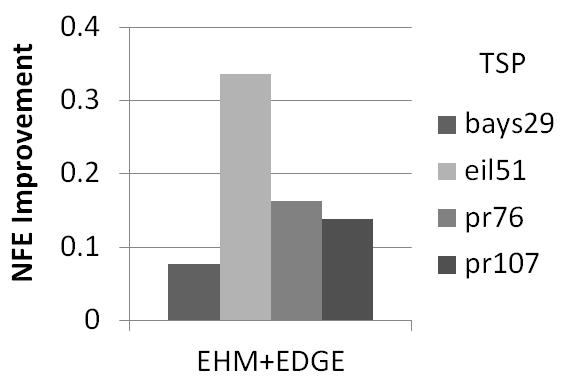
\includegraphics[width=0.5\textwidth]{EHM+edge.png}
        \caption{ Improvements in NFE of EHM with the edge distance } 
        \label{fig:ehbsa_imp}
\end{figure}

For investigating the efficiency of the edge distance, we test EHM and EHM+RTR which uses the edge distance on TSP with the minimum required population size which is the minimum size for solving the objective problem, maximum NFE $E_{max} = \ell\times 40000$ and the number of cut points which is 3, and repeat 20 times respectively. Figure \ref{fig:ehbsa_imp} shows NFE reduced by RTR with the edge distance. 
The results indicate that RTR with the edge distance is able to improve the performance of EHM on TSP. Besides, as the difficulty of permutation problem growing up, the improvement increases. By the way, the problem size of $pr76$ is larger than $eil51$, but the minimum required population size of $pr76$ is smaller than $eil51$. This means that $eil51$ is more difficult problem than $pr76$. 

\subsection*{Node Distance}
The node distance is calculated by each node at different position between two individuals. Let $D_{node} (i,j)$ denote the node distance between the two individuals $i$ and $j$. $D_{node} (i,j)$ is calculated as follows:\[D_{node} (i,j)=\sum_{k=0}^{ell-1} r_{i,j} (k), \]
where $r_{i,j} (k)$ is a function defined as \[r_{i,j} (k)=
\begin{cases}
1,  & \mbox{if }\pi_{k,i}\neq \pi_{k,j} \\
0, & \mbox{otherwise}
\end{cases}
.\] For example, given two individuals $x=(1,2,3,4,5)$ and $y=(5,2,1,3,4)$, the nodes $1$, $3$, $4$ and $5$ are not at the same position in both individuals. Thus, the node distance between $x$ and $y$ is $4$.



\begin{figure}[htbp] 
        \centering
        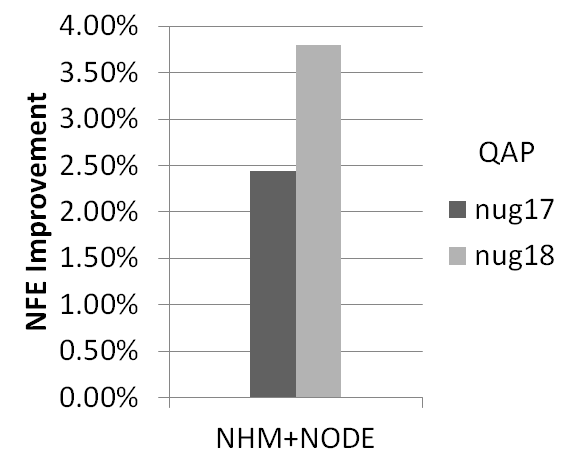
\includegraphics[width=0.5\textwidth]{NHM+node.png}
        \caption{ Improvements in NFE of NHM with the node distance } 
        \label{fig:nhbsa_imp}
\end{figure}


For investigating the efficiency of the node distance, we test NHM and NHM+RTR which uses the node distance on QAP with the minimum required population size, maximum NFE $E_{max} = \ell\times 40000$ and the number of cut points which is 3, and repeat 20 times respectively. Figure \ref{fig:ehbsa_imp} shows NFE reduced by RTR with the node distance. The results indicate that RTR with the node distance is able to improve the performance of NHM on QAP.



\subsection*{Order Distance}
The order distance is calculated by different orders of every node pair between two individuals. Let $D_{order} (i,j)$ represent the order distance between the two individuals $i$ and $j$, and \[OS_i=\lbrace\forall x,y(\pi_x^i,\pi_y^i)| x>y\rbrace\mbox{ be an order set of individual }i.\] The order distance $D_{order} (i,j)$ is calculated as follows:\[D_{order} (i,j)=\binom{\ell}{2}-\vert OS_i\cap OS_j\vert.\]
Consider an example of order distance, two individuals $x=(1,2,3,4,5)$ and $y=(5,2,1,3,4)$ are given, the orders $(1,2)$, $(1,5)$, $(2,5)$, $(3,5)$, $(4,5)$ are not at the intersection of $OS_x$ and $OS_y$. Thus, the order distance between $x$ and $y$ is $2$. 




\begin{figure}[htbp] 
        \centering
        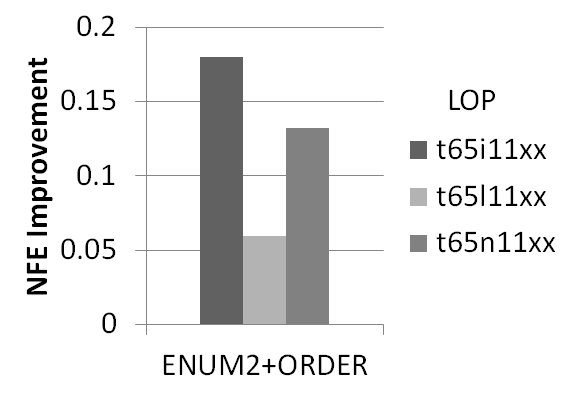
\includegraphics[width=0.5\textwidth]{ENUM2+ORDER.png}
        \caption{ Improvements in NFE of EHM+NHM with the order distance } 
        \label{fig:enum2_imp}
\end{figure}


For investigating the efficiency of the order distance, we test Enum2 and Enum2+RTR which uses the order distance on LOP with the minimum required population size and maximum NFE $E_{max} = \ell\times 40000$, and repeat 20 times respectively. In this experiment, we use the enumeration method to choose model. Figure \ref{fig:enum2_imp} shows NFE reduced by RTR with the order distance. The results indicate that RTR with the order distance is able to improve the performance of Enum2 on LOP. 


\subsection{Essence of Distance-measure Choosing}
This section shows the essence of distance-measure choosing. For the same reason of essence of model adaptation, the mechanism of distance-measure adaptation is necessary. 


For Investigating the essence of distance-measure choosing, we test EHM with the edge distance, EHM with the node distance, NHM with the edge distance and NHM with the edge distance on QAP and TSP. We perform independent 20 runs with maximum NFE $E_{max} = \ell \times 40000$ and the population size $N=\ell\times 2$ for each iteration. The results are shown in Figures \ref{fig:essence2}. As we can see, EHM+RTR with the edge distance outperforms EHM with the node distance, and NHM with the node distance outperforms NHM with the node distance. This means that RTR with the correct distance measure outperforms that with wrong distance measure but model choosing is more important than distance-measure choosing on permutation problems.

\begin{figure}[htbp] 
        \centering
        \begin{subfigure}{1\textwidth}
            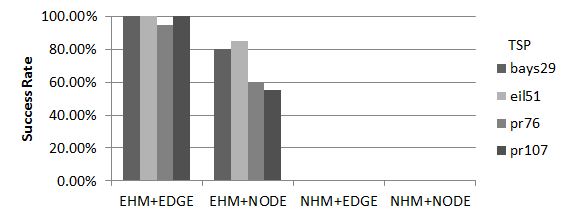
\includegraphics[width=\textwidth]{essenceTSP.png}
            \caption{  Success rates of the algorithms on TSP } 
        \end{subfigure}

        \begin{subfigure}{1\textwidth} 
            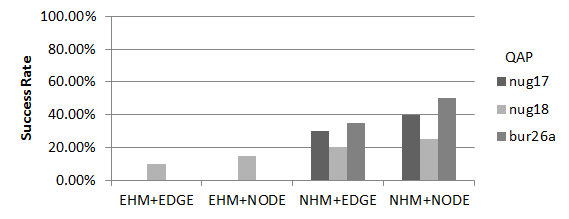
\includegraphics[width=\textwidth]{essenceQAP.png}
            \caption{ Success rates of the algorithms on QAP}
        \end{subfigure}
        
        \caption{ Results of EHM+EDGE, EHM+NODE, NHM+EDGE and NHM+NODE on TSP and QAP } 
        \label{fig:essence2}
\end{figure}


In another experiment, we choose the edge distance with the probability $p$ and choose the node distance with the probability $1-p$ at each generation, and use enumeration method to choose EHM or NHM. The probability $p$ starts from 0.0 to 1.0 and increases 0.1 by each iteration. the instances of LOP are used : $t65i11x$ and $t65n11x$ from LOLIB. We perform independent 10 runs with the maximum NFE $E_{max} = \ell \times 40000$ for each iteration. The results are shown in Figure \ref{fig:sweep_imp}. We can find that the best performance is not at maximum or minimum of $p$. This experiment indicates that mixing different distance measure can solve permutation problems more effectively.



\begin{figure}[htbp] 
        \centering
        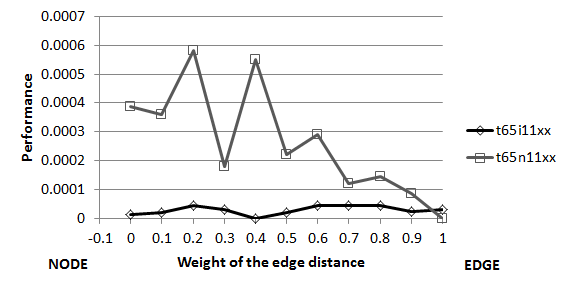
\includegraphics[width=0.9\textwidth]{essence.png}
        \caption{ Success rates of EHM+NHM with the sweeping probability choosing the node distance. } 
        \label{fig:sweep_imp}
\end{figure}


\subsection{Model-associated Method}
In this section, we introduce the model-associated method. The model-associated method is a method of distance-measure choosing. In each RTR, the model-associated method chooses the corresponding distance measure with the semantic model which selected on model-choosing phase. For example, let $MS=\langle m_1 , m_2, ..., m_{N_M}\rangle$ be an ordered set of semantic models and $DS=\langle d_1 , d_2, ..., d_{N_M}\rangle$ be an ordered set of distance measures, where ${N_M}$ is the number of models, $m_i$ represents the semantic model $i$ and $d_i$ denotes the corresponding distance measure of the semantic model $i$. Table \ref{tb:model_distance} shows the semantic models and their corresponding distance measures in our work.


\begin{table}[htbp]
    \centering
    \begin{tabular}{|l|l|}
    \hline
    \textbf{Semantic Models}       & \textbf{Corresponding Distance}  \\ \hline
    \textbf{NHM} & Node Distance    	 \\ \hline
    \textbf{EHM} & Edge Distance  	\\ \hline
    \textbf{PL} & Order Distance  	\\ \hline
  
    \end{tabular} 
    \caption{Semantic models and their corresponding distance measures}
    \label{tb:model_distance}
\end{table}

\begin{figure}[htbp] 
        \centering
        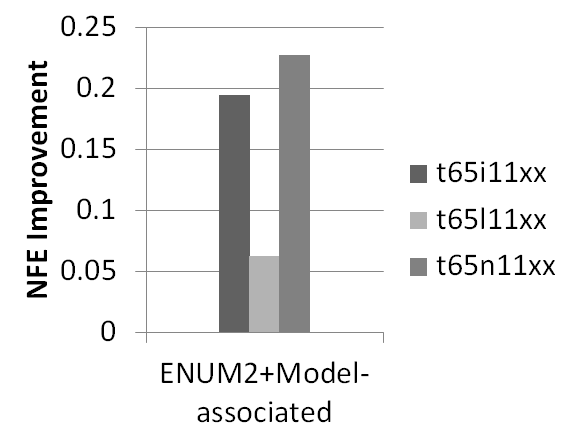
\includegraphics[width=0.5\textwidth]{ENUM2+model.png}
        \caption{ Improvements in NFE of RTR with the model-associated method on LOP } 
        \label{fig:enum2_model}
\end{figure}

To investigate the performance of the model-associated method, we test EHM+NHM and EHM+NHM with the model-associated method on LOP with the minimum required population size, maximum NFE $E_{max} = \ell\times 40000$ and the number of cut points which is 3, and repeat 20 times respectively. In this experiment, we use enumeration method to choose EHM or NHM. The results are shown in Figure \ref{fig:enum2_model}. The results shows that RTR with the model-associated method is able to improve the performance of EHM+NHM on LOP. Comparing with the experimental results of the order distance, the performance of RTR with the model-associated method is close to that with the order distance. 

\subsection*{Reward Policy}

Based on the assumption that the successes of the replacements with RTR keeps more information, we modify the reward policy of model adaptation. We change the reward policy $r$ from \[r=
\begin{cases}
1,  & \mbox{if the new individual is better than template~~~~~~~~~~~~~~~~~~~~ }\\
0, & \mbox{otherwise}
\end{cases}
\]to\[r=
\begin{cases}
1,  & \mbox{if the new individual is better than the one choosen by RTR}\\
0, & \mbox{otherwise.}
\end{cases}
\]
To investigate the performance of the new reward policy, we test MABMA with the model-associated method using the original reward policy and the new reward policy respectively. In this experiment, EHM and NHM are used, the population size $N$ is $\ell$ and maximum NFE $E_{max}$ is $\ell\times 40000$. We select 50 instances of TSP for testing which can be divided into two parts. One part consists of 24 instances which were used in~\cite{ceberio2012review} : $bays29$, $berlin52$, $burma14$, $ch130$, $dantzig42$, $eil51$, $eil76$, $eil101$, $fri26$, $gr17$, $gr24$, $gr48$, $gr96$, $gr137$, $hk48$, $pr76$, $pr107$, $pr124$, $pr136$, $rat99$, $st70$, $swiss42$, $ulysses16$, $ulysses22$. The remaining instances are chosen by considering small, medium and large problem size as follows:
\begin{itemize}
    \item Small: $br17$, $gr21$, $bayg29$, $ftv33$, $ftv35$, $ftv38$, $p43$, $ftv47$, $att48$, $ry48p$,
    \item Medium: $ft53$, $ftv55$, $brazil58$, $ftv64$, $ft70$, $ftv70$ and
    \item Large: $kroA100$,	$kroB100$,	$kroC100$,	$kroD100$,	$kroE100$,	$gr120$,	$bier127$,	$pr144$,	$ch150$.
\end{itemize}
We compare the usage of the correct semantic model--EHM at $3000$-th generation and the fitness on termination. The results are shown in Table \ref{tb:reward}. This experiment indicates that the new reward policy outperform the original reward policy. As we can see, the usage of EHM with the new reward policy is higher than with the original reward policy at $3000$-th generation. EHM would keep higher usage for a long time until the successful replacement is hard for both semantic models. This is means that the semantic RTR is helpful for the model adaptation.

\begin{table}[htbp]
    \centering
    \begin{tabular}{|l|l|l|}
    \hline
    \textbf{Reward Policy}       &\textbf{Higher usage of EHM}       & \textbf{Achieving higher fitness}  \\ \hline
    \textbf{The original reward} & 21/50 & 14/50   	 \\ \hline
    \textbf{The modified reward} & 29/50 & 36/50	\\ \hline
    \end{tabular} 
    \caption{The result of comparing between the original reward and the modified reward on TSP}
    \label{tb:reward}
\end{table}
\subsection*{Window Size}

In this section, we investigate the window size of RTR on permutation problems. For this purpose, we test EHM with the edge distance, NHM with the node distance and PL with the order distance on TSP, QAP and LOP respectively. The different window sizes and the corresponding distance measures are used, the population size $N$ is $\ell$, maximum NFE $E_{max}$ is $\ell\times 5000$, and each algorithm repeats three times. We select 20 instances which were used in~\cite{ceberio2012review} for each problem type:
\begin{itemize}
    \item TSP: $bays29$, $ berlin52$, $ ch130$, $ dantzig42$, $eil51$, $ eil76$, $eil101$, $ fri26$, $ gr17$, $gr24$, $ gr48$, $ gr96$, $ gr137$, $ hk48$, $ pr76$, $ pr107$, $pr124$, $ pr136$, $rat99$, $st70$, $swiss42$, 
    \item QAP: $bur26a$, $ bur26b$, $ bur26c$, $bur26d$, $ nug17$, $nug18$, $ nug20$, $ nug21$, $tai10a$, $tai10b$, $tai12a$, $tai12b$, $tai15a$, $tai15b$, $tai20a$, $tai25a$, $tai30a$, $tai35a$, $tai35b$, $tai40a$ and
    \item LOP: $t75i11xx$, $t65f11xx$, $ t65b11xx$, $ t65d11xx$, $ t65i11xx$, $t65l11xx$, $ t65n11xx$, $ t65w11xx$, $ t69r11xx$, $t70b11xx$, $ t70d11xx$, $ t70d11xxb$, $be75eec$, $ be75np$, $ be75oi$, $ tiw56n54$, $tiw56n58$, $ tiw56n66$, $stabu70$, $ stabu74$, $ usa70$.
\end{itemize} 
 In the experiments, we keep the template in the window of RTR at each generation. The performance measure employed in our study is the number of best rank which means that the algorithm with the size has best performance of NFE and fitness.

\begin{figure}[htbp] 
        \centering
        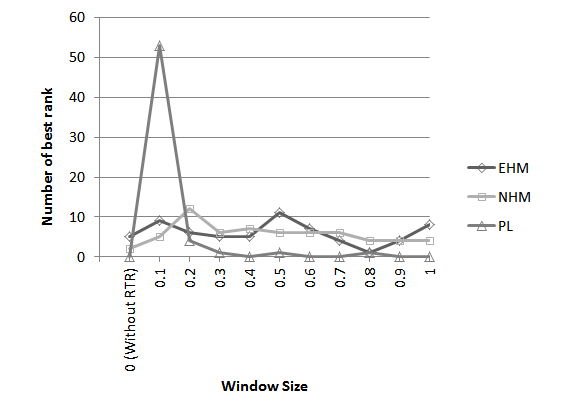
\includegraphics[width=1\textwidth]{window_size.png}
        \caption{ Rank results of EHM, NHM and PL with different window sizes } 
        \label{fig:w_size}
\end{figure}



The results are shown in Figure \ref{fig:w_size}. As we can see, the point of EHM with the window size $w=\ell\times 0.5$ overall has the lowest ARPD for all instances. The point of NHM with the window size $w=\ell\times 0.2$ overall has the lowest ARPD for all instances for NHM, and the point of PL with the window size $w=\ell\times 0.1$ overall has the lowest ARPD for all instances for PL. The point with window size $w=0$ is identical to the algorithm without RTR in our experiments. Finally, we give the suggested settings of the window size as follows:
\begin{itemize}
    \item the window size for EHM is $\ell\times 0.5$,
    \item the window size for NHM is $\ell\times 0.2$
    \item and the window size for PL is $\ell\times 0.1$.
\end{itemize}




In another experiment, we investigate whether the template should be included in the window of RTR. The results are shown in Figure \ref{fig:w_template}. The performance measure employed in our study is the average relative percentage deviation (ARPD):\[ARPD=\left|\left(\sum_{i=1}^{runs}\frac{Best-Result_i\times 100}{Best} \times \frac{1}{runs}\right)\right|\], where $Result_i$ is the best fitness found by the algorithm in the $i-th$ repetition, $Best$ is the fitness of the best known solution and $runs$ is 3 in this experiment. The performance of including template in the window outperforms. This is because of the information contained in template. The template is the lower bound of RTR.


\begin{figure}[htbp] 
        \centering
        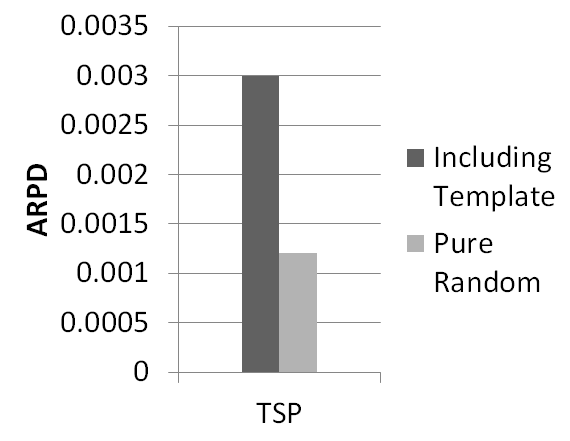
\includegraphics[width=0.5\textwidth]{include_template.png}
            \caption{ARPD results of the algorithm including the template in window and pure random picking} 
        \label{fig:w_template}
\end{figure}
\subsection{Empirical Study}
In this section, we investigate the performance of RTR with the model-associated method. For this purpose, we perform MABMA with the model-associated method and the original. The experimental settings are as follows:
\begin{itemize}
    \item repeat 20 times,
    \item EHM, NHM and PL are used,
    \item the number of cut points is 3 for template,
    \item maximum NFE $E_{max}$ is $\ell \times 40000$,
    \item the population size $N$ is $\ell \times 2$,
    \item the new reward policy is used,
    \item the window size is $\ell\times 0.5$ for EHM, $\ell\times 0.2$ for NHM and $\ell\times 0.1$ for PL,
    \item the benchmark instances of TSP :$bays29$, $eil51$, $pr76$, $kroA100$ and $pr107$ are used,
    \item the benchmark instances of QAP :$nug17$, $nug18$, $bur26a$, $ tai30b$ and $bur26b$ are used,
    \item the benchmark instances of LOP :$t65b11x$, $t65b11x$, $t65d11x$, $t65f11x$ and $t65n11x$ are used,
    \item the benchmark instances of CVRP $:A-n32-k5$, $A-n33-k5$, $A-n33-k6$, $A-n34-k5$ and $A-n36-k5$ are used
    \item and the benchmark instances of FSSP :$20\_5\_01\_ta001$, $20\_10\_01\_ta011$, $20\_20\_01\_ta021$, $50\_5\_01\_ta031$ and $50\_10\_01\_ta041$ are used.
\end{itemize}

Figure \ref{fig:arpdi} shows the ARPD results of MABMA and MABMA with the model-associated method. Comparing the performance of our proposed method with the original MABMA, the ARRD results of our proposed method are smaller than the ARRD results of original MABMA on each problem, in other words, MABMA with the model-associated method outperforms the original. This indicates that our proposed method is close to the best performing model with RTR and outperforms any single model without that in this work.

%Combining RTR, distance-measure choosing, the modified reward policy and the suggested window sizes, our proposed method is close to the  best performing model with RTR and outperforms any single model without that in this work. 
\begin{figure}[htbp] 
        \centering
        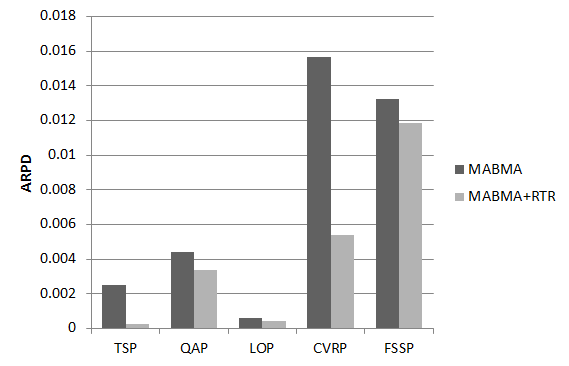
\includegraphics[width=1\textwidth]{arpdi.png}
        \caption{ ARPD results of MABMA and MABMA with the model-associated method on TSP, QAP, LOP, CVRP and FSSP. } 
        \label{fig:arpdi}
\end{figure}



\section{Replacement Strategy}
\label{ch:replacement_strategy}

This chapter focuses on replacement strategy and give a brief introduction to the restricted tournament replacement (RTR). This chapter also shows the effects of RTR, the essence of distance-measure adaptation and the method of distance-measure adaptation. To reduce NFE, we use RTR to decide which individual should be replaced or be preserved. Thus, we define three types of distance measures for RTR on the permutation problems.




\subsection{Restricted Tournament Replacement}
The restricted tournament replacement (RTR) is a commonly used niching technique in the field of EDAs. RTR is also known as restricted tournament selection (RTS) which is first proposed in \citep{harik1995rts}. RTR uses the tournament strategy to decide the part which get to move on to the next generation. We present the process of RTR in algorithm \ref{alg:RTR_algorithm}, where the $Distance$ function is usually the Hamming distance in binary problems. However, Hamming distance is not suitable for the permutation problems. Thus, we define new distance for the permutation problems by characteristics of the permutation problems. In our work, the window size $w$ is suggested to set to $L/3$.


\begin{algorithm}[htbp]
    \SetKwRepeat{doWhile}{do}{while}
    \KwIn{The original population $X=\lbrace x_1, x_2, ..., x_{n-1}\rbrace$\;
    The offspring population $Y$\;
    The window size $w$\; }
    \KwOut{The population $X$ of the next generation;}
    \For{ $y\in Y$ }
    {
        Choose a random subset $S =\lbrace s_0, s_1, ..., s_{w-1}\rbrace (0\leq s_i <n)$\;
        Find the $x_{s_i}$ in $\mathop{\argmin}_{{s_i} \in S} Distance(x_{s_i},y)$\;
        \If{$Fitness(y)>Fitness(x_{s_i})$}      {
        $x_{s_i} \leftarrow y$;
        }
        
    }
    return $X$\;
    \caption{The algorithm of RTR}
    \label{alg:RTR_algorithm}
\end{algorithm}


\subsection{Distance Metric}

This subsection shows three types of distance measures for RTR on the permutation problems: edge distance, node distance and order distance. We define three distance measures by considering semantics of permutation problems.
\subsection*{Edge Distance}


An edge is connection between two nodes. The edge distance is calculated by different edge between two individuals. Let $D_{edge} (i,j)$ denote the edge distance between the two individuals $i$ and $j$, and \[ES_i=\lbrace\forall k(\pi_{(k\ mod\ L),i}, \pi_{(k+1\ mod\ L),i})\rbrace\mbox{ is an edge set of individual }i.\] Thus, $D_{edge} (i,j)$ is calculated as follows:\[D_{edge} (i,j)=L-\vert ES_i\cap ES_j\vert.\]

\begin{figure}[htbp] 
        \centering
        \begin{subfigure}{0.49\textwidth}
            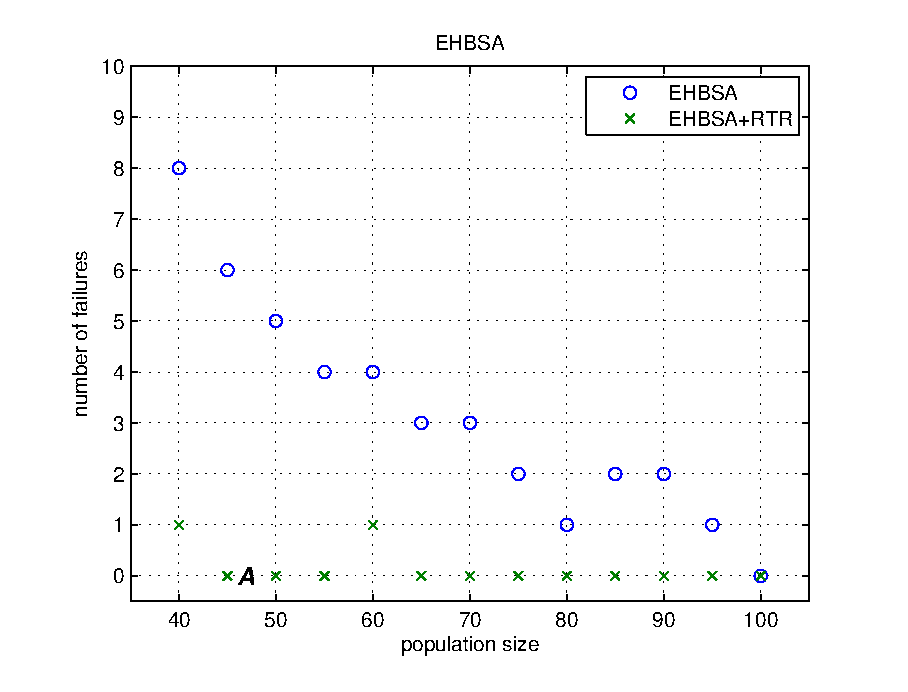
\includegraphics[width=\textwidth]{pf_a.eps}
            \caption{PopulationSize-Failures} 
        \end{subfigure}
        \begin{subfigure}{0.49\textwidth} 
            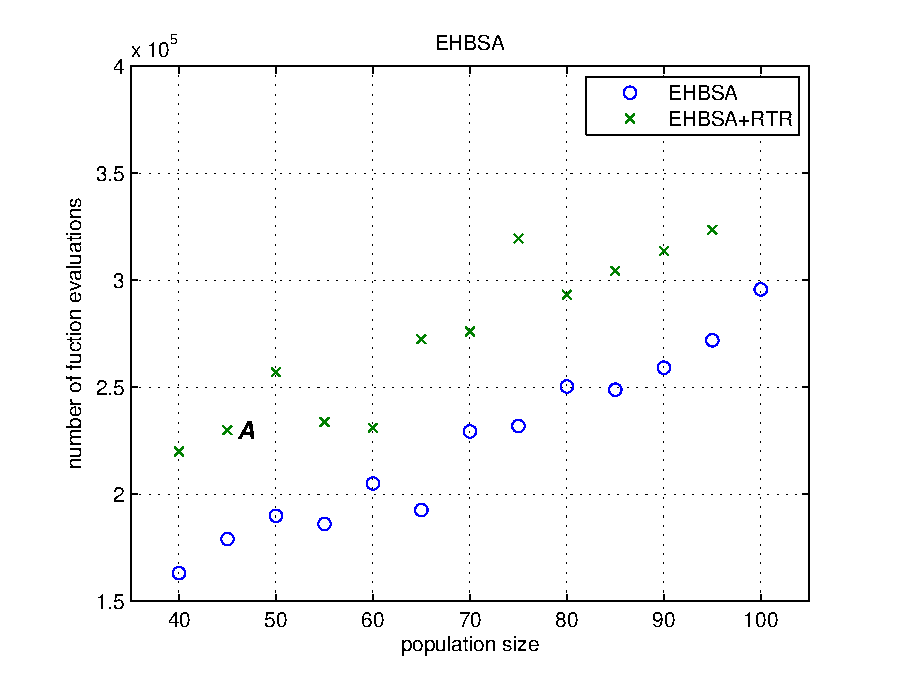
\includegraphics[width=\textwidth]{pn_a.eps}
            \caption{PopulationSize-$N_{fe}$}
        \end{subfigure}

        \caption{(Temp)Results of EHBSA on benchmark $eil51$ with template technique and $B_{ratio}=0.00$.  } 
        \label{fig:ehbsa_pf}
\end{figure}

We test EHBSA and EHBSA+RTR which uses the edge distance with different population size 20 times on benchmark $eil51$ respectively. The results are shown in Figure \ref{fig:ehbsa_pf}. The number of function evaluations increases and number of failures decreases as population size growing up. Comparing the performance of EHBSA and EHBSA+RTR, number of function evaluations of EHBSA+RTR is larger than EHBSA, but number of failures of EHBSA+RTR is the smaller than EHBSA. The point A represent the best performance of EHBSA+RTR, and it is smallest number of function evaluations among all lowest failure rate points in Figure \ref{fig:ehbsa_pf}. We get the conclusion that EHBSA+RTR with minimum required population size outperforms EHBSA. Edge distance is useful on TSP.

\subsection*{Node Distance}
The node distance is calculated by each node at different position between two individuals. Let $D_{node} (i,j)$ denote the node distance between the two individuals $i$ and $j$. $D_{node} (i,j)$ is calculated as follows:\[D_{node} (i,j)=\sum_{k=0}^{ell-1} r_{i,j} (k), \]
where $r_{i,j} (k)$ is a function defined as \[r_{i,j} (k)=
\begin{cases}
1,  & \mbox{if }\pi_{k,i}\neq \pi_{k,j} \\
0, & \mbox{otherwise}
\end{cases}
.\]


\begin{figure}[htbp] 
        \centering
        \begin{subfigure}{0.49\textwidth}
            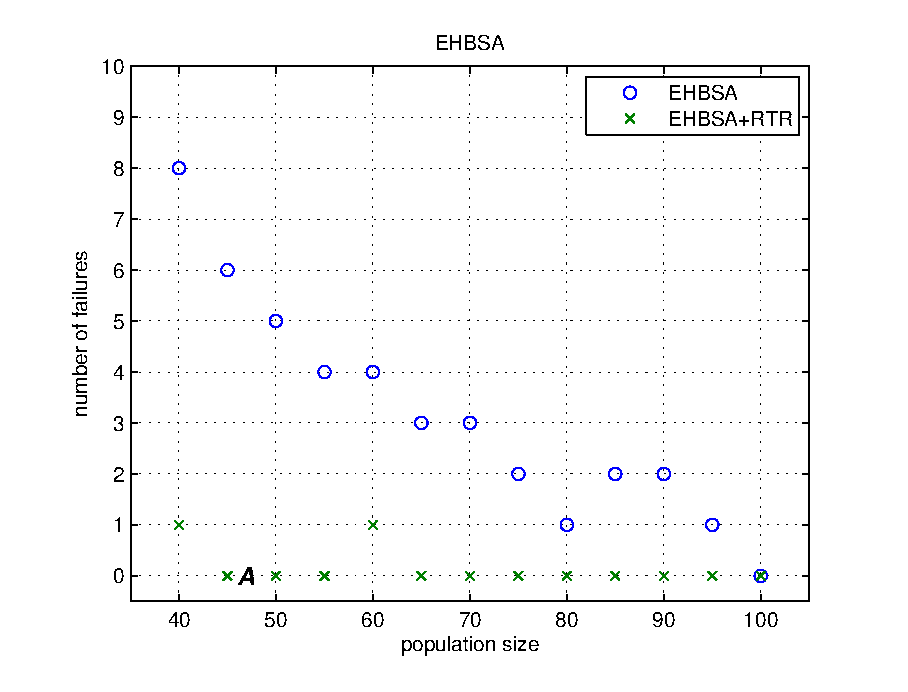
\includegraphics[width=\textwidth]{pf_a.eps}
            \caption{PopulationSize-Failures} 
        \end{subfigure}
        \begin{subfigure}{0.49\textwidth} 
            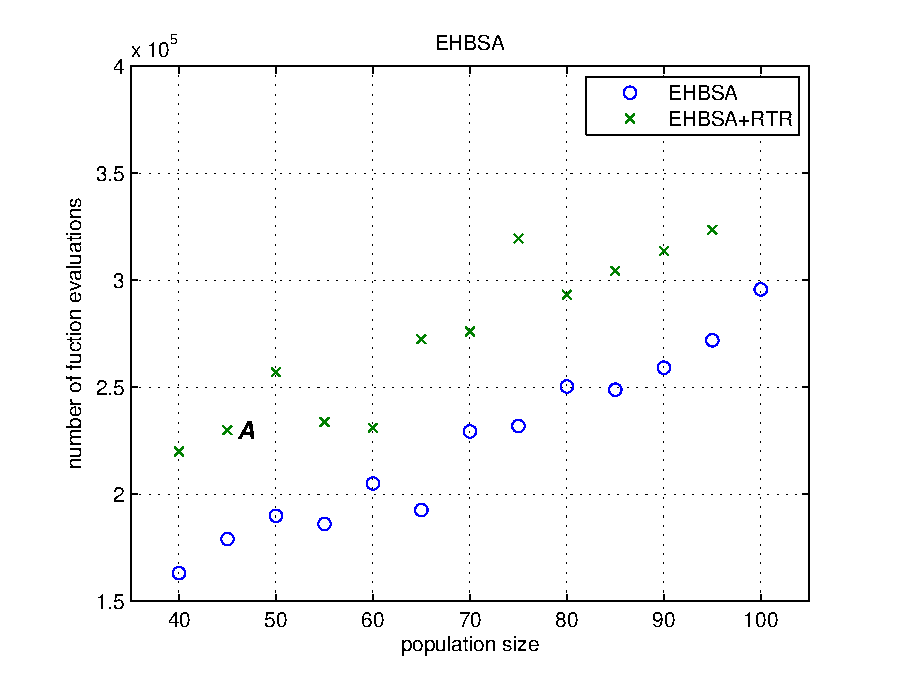
\includegraphics[width=\textwidth]{pn_a.eps}
            \caption{PopulationSize-$N_{fe}$}
        \end{subfigure}

        \caption{(Temp)Results of NHBSA on benchmark $ta031$ with template technique and $B_{ratio}=0.00$.  } 
        \label{fig:nhbsa_pf}
\end{figure}

We test NHBSA and NHBSA+RTR which uses the node distance with different population size 20 times on FSSP respectively. The results are shown in Figure \ref{fig:nhbsa_pf}. This experiment indicates that NHBSA+RTR with minimum required population size outperforms NHBSA, and node distance is useful on FSSP.



\subsection*{Order Distance}
The order distance is calculated by different orders of every node pair between two individuals. Let $D_{order} (i,j)$ denote the order distance between the two individuals $i$ and $j$. $D_{order} (i,j)$ is calculated as follows:\[D_{order} (i,j)=\sum_u \sum_v \delta_{i,j}(u,v),\]
where $\delta_{i,j} (u,v)$ is a function defined as \[\delta_{i,j} (u,v)=
\begin{cases}
0,  & \mbox{if }H_{\pi_{u}},i>H_{\pi_{v}},i\mbox{ and } }H_{\pi_{u}},j>H_{\pi_{v}},j}  \\
1, & \mbox{otherwise.}
\end{cases}
\]
In the above, $H_{\pi_{x}},i$ denotes $\pi_{x}$ of individual $i$.



\begin{figure}[htbp] 
        \centering
        \begin{subfigure}{0.49\textwidth}
            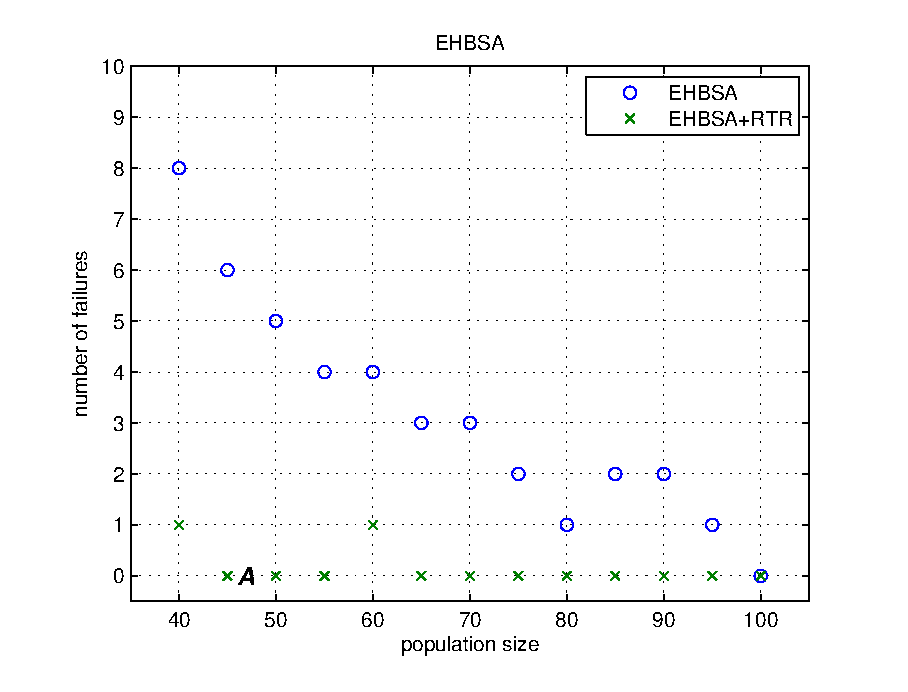
\includegraphics[width=\textwidth]{pf_a.eps}
            \caption{PopulationSize-Failures} 
        \end{subfigure}
        \begin{subfigure}{0.49\textwidth} 
            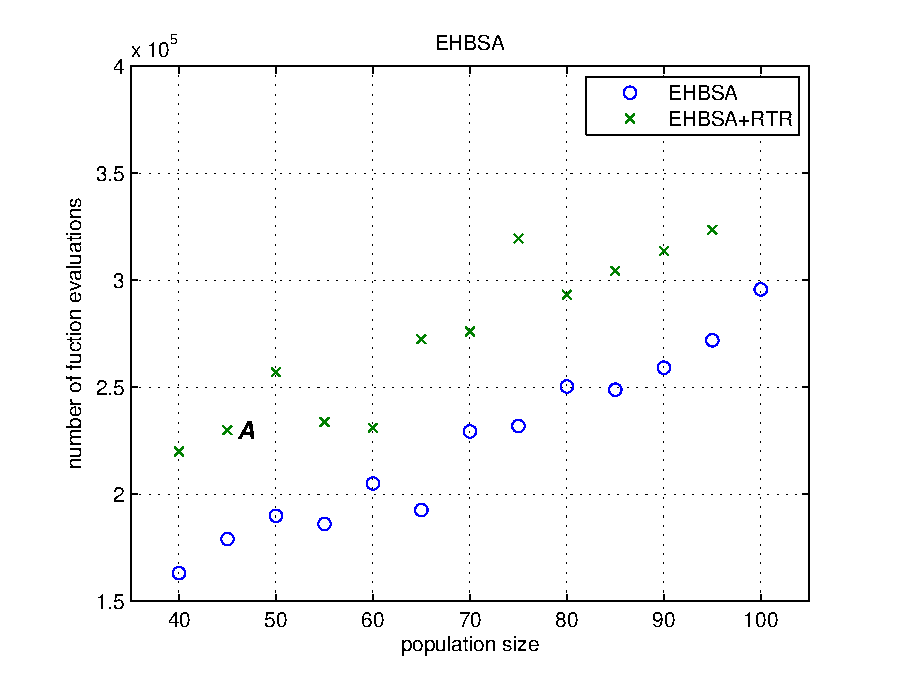
\includegraphics[width=\textwidth]{pn_a.eps}
            \caption{PopulationSize-$N_{fe}$}
        \end{subfigure}

        \caption{(Temp)Results of Enum2(EHBSA, NHBSA) on benchmark $t65i11xx$ with template technique and $B_{ratio}=0.000$.  } 
        \label{fig:order_pf}
\end{figure}


We test Enum2 and Enum2+RTR which uses the order distance with different population size 20 times on LOP respectively. The results are shown in Figure \ref{fig:nhbsa_pf}. This experiment indicates that Enum2+RTR can solve LOP more effective than Enum2, and order distance is useful on LOP.


\subsection{Essence of Distance-measure Adaptation}
This section shows the essence of distance-measure adaptation. For the same reason of essence of model adaptation(chapter \ref{ch:essence_of_adaptation}), the mechanism of distance-measure adaptation is necessary. Due to the different semantics of the permutation problems , the best fit distance measure is non-trivial.

In our experiments, we choose edge distance with the probability $p$ and choose node distance with the probability $1-p$ in each generation. The probability $p$ starts from 0.0 to 1.0 and increases 0.1 by each iteration. the instances of LOP are used : $t65b11x,t65d11x,t65f11x$ and $t65n11x$ from LOLIB. We perform independent 20 runs with the the NFE limit $E_{max} = L \times 40000$ for each iteration.
%\begin{itemize}
    %\item repeat 20 times,
    %\item test enumeration method( the EHM and the NHM are used) on LOP,
    %\item RTR is used,
    %\item the bias ratio $B_{ratio} = 0.0000$,
    %\item the NFE $E_{max} = L \times 40000$,
    %\item the edge distance and the node distance are used,
    %\item the probability $p$ starts from 0.0 to 1.0 and increases 0.1 by each iteration,
    %\item template technique is used ,
    %\item the instance of LOP : $t65b11x,t65d11x,t65f11x$ and $t65n11x$ from LOLIB ,
    %\item the cut-point number is 3 for template.
%\end{itemize}


\begin{figure}[htbp] 
        \centering
        \begin{subfigure}{0.49\textwidth}
            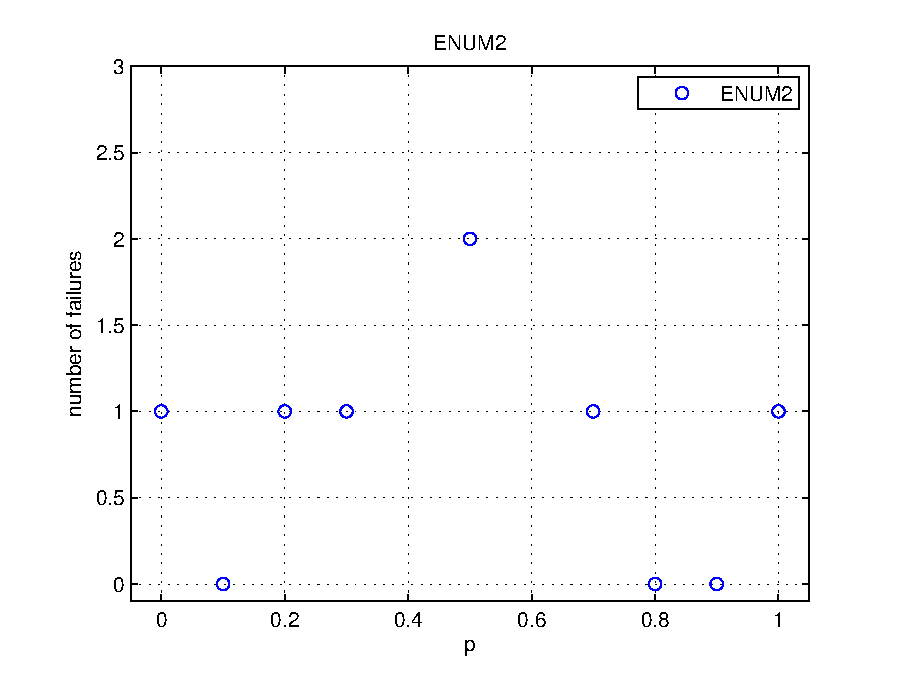
\includegraphics[width=\textwidth]{enum2_f.eps}
            \caption{p-Failures} 
        \end{subfigure}
        \begin{subfigure}{0.49\textwidth} 
            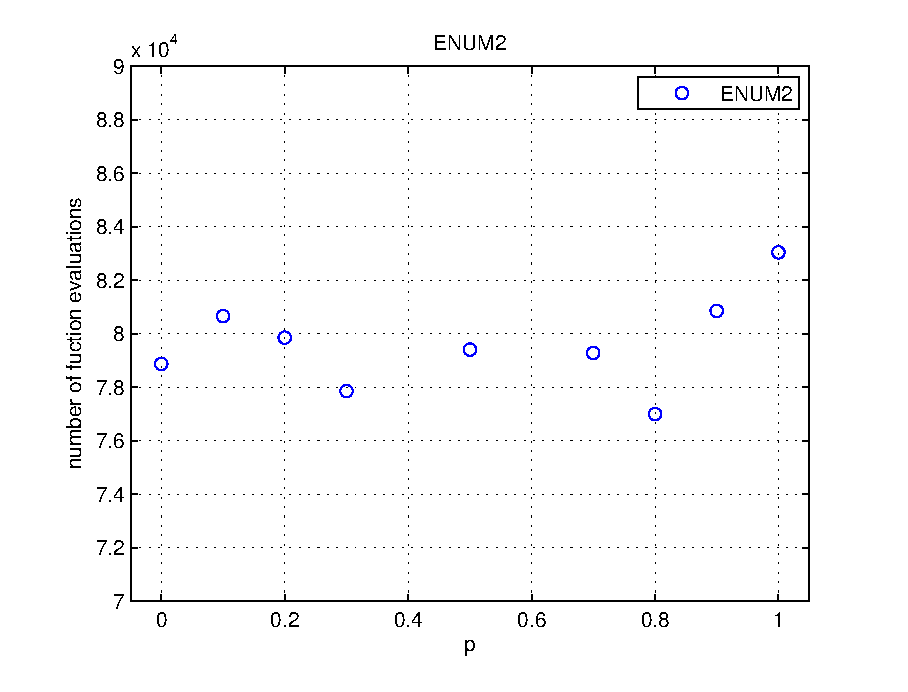
\includegraphics[width=\textwidth]{enum2_n.eps}
            \caption{p-$N_{fe}$}
        \end{subfigure}

        \caption{(Temp)Results of enumeration method on LOP with RTR by using the edge distance and node distance.  } 
        \label{fig:enum_pf}
\end{figure}

Figure \ref{fig:enum_pf} shows NFE and the number of failures of each probability $p$. We can find that the best performance is not at two ends of range of $p$. Therefore, best distance measure is not fixed on node distance or edge distance. This experiment indicates that mixing different distance measure can solve the permutation problems more effectively.

\subsection{Model-associated Method}
The model-associated method is a method of distance-measure adaptation. In each RTR, the model-associated method chooses the corresponding distance measure with selected model on model choosing phase. For example, let $MS=\langle m_1 , m_2, ..., m_{N_M}\rangle$ be an ordered set of models and $DS=\langle d_1 , d_2, ..., d_{N_M}\rangle$ be an ordered set of distance measures, where ${N_M}$ is the number of models. Besides, $m_i$ represents model $i$, and $d_i$ denotes the corresponding distance measure of model $i$. the model-associated method chooses the distance measure corresponding to the selected model in the model choosing phase. Table \ref{tb:model_distance} shows the models and their corresponding distance measures.


\begin{table}[htbp]
    \centering
    \begin{tabular}{|l|l|}
    \hline
    \textbf{Semantic Models}       & \textbf{Corresponding Distance}  \\ \hline
    \textbf{NHM} & node     	 \\ \hline
    \textbf{EHM} & edge   	\\ \hline
    \textbf{the PL model} & order   	\\ \hline
  
    \end{tabular} 
    \caption{Corresponding distance measures of models}
    \label{tb:model_distance}
\end{table}

To investigate the performance of the model-associated method, we test Enum2+RTR by using the edge distance, the node distance and the model-associated method on LOP with the NFE limit $E_{max} = L \times 40000$. %The experiment settings are as follows:
%\begin{itemize}
    %\item repeat 20 times,
    %\item test enumeration method( the EHM and the NHM are used) on LOP,
    %\item RTR is used,
    %\item the bias ratio $B_{ratio} = 0.0000$,
    %\item the NFE $E_{max} = L \times 40000$,
    %\item the edge distance , the node distance and the model-associated method are used,
    %\item template technique is used ,
    %\item the instance of LOP : $t65b11x,t65d11x,t65f11x$ and $t65n11x$ from LOLIB ,
    %\item the cut-point number is 3 for template.
%\end{itemize}
\subsection{Reward Policy}
\subsection{Window Size}
\subsection{Empirical Study}
This section shows the performance of MABMA+RTR on the different permutation problems. For comparison, MABMA-UCB, MABMA-UCBT, MABMA-UCB+RTR, MABMA-UCBT+RTR are tested on LOP,TSP,QAP and VRPTW. In the experiment of the model-associated method, EHM, NHM and the PL model are used. For each instance, we perform independent 20 runs with the NFE limit $E_{max} = L \times 40000$.
%\begin{itemize}
    %\item repeat 20 times,
    %\item test MABMA(EHBSA, NHBSA and PLEDA are used) on LOP,TSP,FSSP and CVRP,
    %\item RTR is used,
    %\item the bias ratio $B_{ratio} = 0.0000$,
    %\item the NFE $E_{max} = L \times 40000$,
    %\item the model-associated method is used,
    %\item template technique is used ,
    %\item the cut-point number is 3 for template.
%\end{itemize}



\section{Conclusion}
%\section{Conclusion}
\label{ch:conclusion}

This paper proposed a model adaptation framework of different models of EDAs for the permutation optimization problems, three distance measure for the RTR and the method of distance-measure adaptation. We stated by means of examples of the permutation problems that, although all solutions are encoded as permutations, their semantics change from one problem to another. Several permutation models using different strategies are illustrated. They showed promising results, but each model can only deal with some parts of the permutation problems effectively. To achieve best performance, choosing dedicated models for specific problem is critical. The semantics of the permutation problems may out of the capability of a model. As a consequence, the model adaptation is essential. For the same reason, the distance-measure adaptation is essential, too.

Experimental results indicates that the method of model adaptation and the method of distance-measure adaptation are promising. Several approaches to achieve model adaptation, three distance measure and the method of distance-measure adaptation were proposed. In order to evaluate the efficiency, they were tested on several well-known permutation problems,including the linear ordering problem, the permutation flow-shop scheduling problem, the capacitated vehicle routing problem and the traveling salesman problem. Experimental results revealed that the multi-armed bandit based model adaptation (MABMA) can achieve better performance than others do. The MABMA can achieve better performance than single model EDAs on complicated permutation problem, and close to the single model EDAs on the problems having dedicated model. Besides, the RTR is effective to improve the performance on the permutation problems.

As for future work, we investigate the techniques learning the needs of different models and distance measures in a permutation segment. Although the model adaptation can deal with more permutation problem, some problems shows more complicated semantics like the vehicle routing problem with time window (VRPTW). In different segment of the permutation in VRPTW, different model is necessary. Also, we are interested in developing the mechanism which can select the best fit model.
%\input{acknowledge}


\small
%\bibliographystyle{bstutf8}

\bibliographystyle{apalike}
\bibliography{thesis}


\end{document}
